\chapter{BBAutoTune}

\label{Chapter4}

\section{Overview}

The purpose of BBAutoTune is to find the correct combination of physics parameters such that the motion of a simulated robot is indistinguishable from its real-world counterpart. Components of BBAutoTune include a genetic algorithm, database manager, a graphical user interface (GUI) panel, and an external progress monitor which tracks various metrics of the running genetic algorithm.  

\section{Implementation}

BBAutoTune's implementation builds off a 3D content creation platform known as Blender. Blender's various features allow one to author static or real-time interactive 3D content. Figure \ref{fig:blender} shows Blender's GUI. Most of the components to BBAutoTune run inside of Blender itself with the exception of the external GA monitor. Blender's API uses the Python programming language and thus BBAutoTune was written entirely in Python.

\begin{figure}[htbp]
\centering
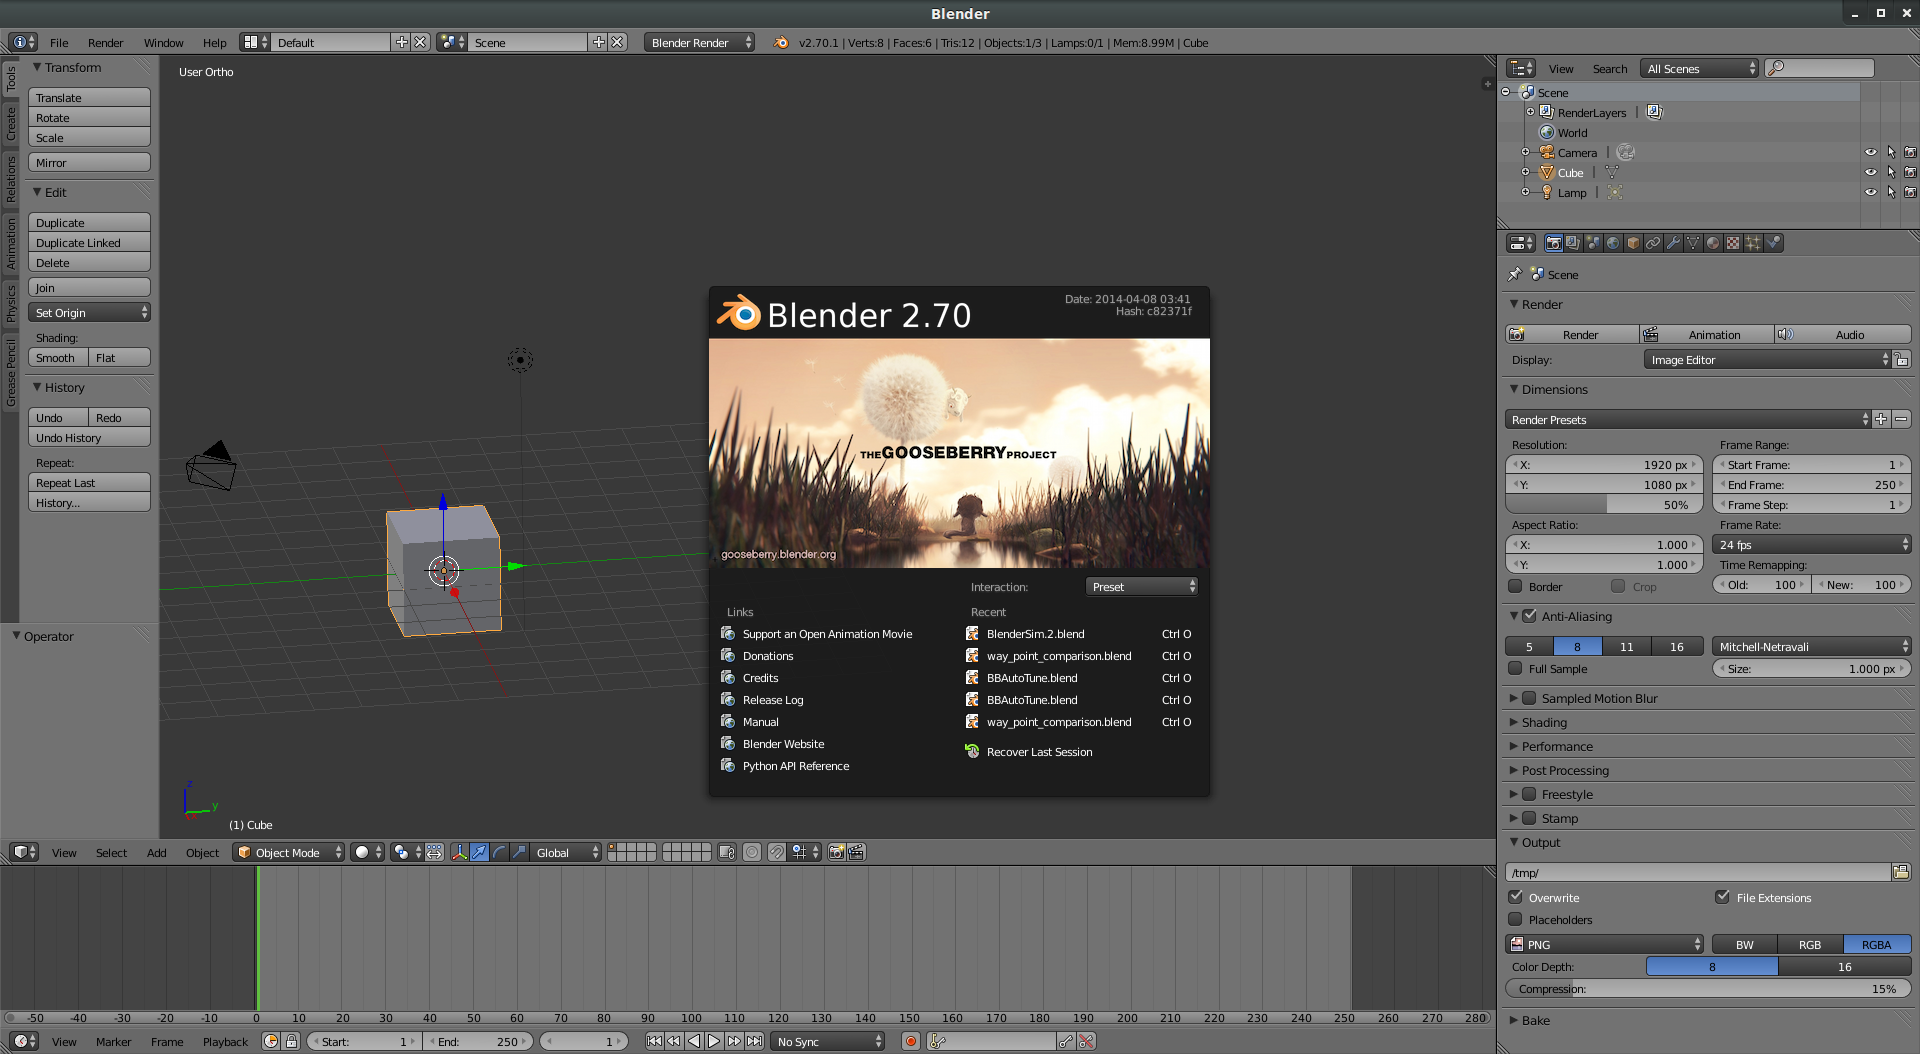
\includegraphics[width=6in]{../Figures/Chapter4/blender.png}
\rule{35em}{0.5pt}
\caption[Blender's Interface]{The Blender interface.}
\label{fig:blender}
\end{figure}

\subsection{Surveyor SRV-1 Blackfin 3D Model}

The robot used during experimentation was a 3D model of the Surveyor SRV-1 Blackfin. This model is dimensionally and aesthetically based on the real robot. The extents of the model are $17.64cm\times14.53cm\times14.33cm$ including the Braille hat that rests above the body of the robot \cite{sklar-et-al-arms:2011}. The base and the wheels are the only physics based objects on the model with the wheels being connected to the base via a rigid body hinge joint. See Figure \ref{fig:srv1_3d_model}. The robot's base was centered at the world origin and the robot was faced down the global positive x-axis. All wheel geometry origins had a global z-axis position of 0.0 and were placed $1.37cm$ above the floor.   

\begin{figure}[htbp]
\centering
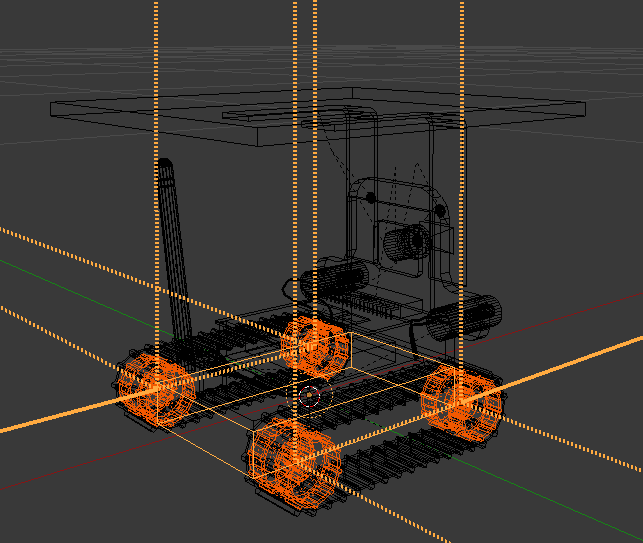
\includegraphics[scale=0.5]{../Figures/Chapter4/srv1.png}
\rule{35em}{0.5pt}
\caption[SRV-1 3D Model]{The 3D model of the Surveyor SRV-1 Blackfin with the wheels connected to the base via rigid body hinge joints.}
\label{fig:srv1_3d_model}
\end{figure}

\subsection{GUI}

Blender's GUI can be extended via its Python API. BBAutoTune adds a custom panel to Blender that allows the user to specify certain parameters pertaining to the GA and the overall tuning loop. Once the user specifies their preferred parameters, they press start to begin the tuning process. After pressing start, BBAutoTune will continue to run until the GA has reached the maximum number of generations specified. See Figure \ref{fig:bbautotune_gui}. 

\begin{figure}[htbp]
\centering
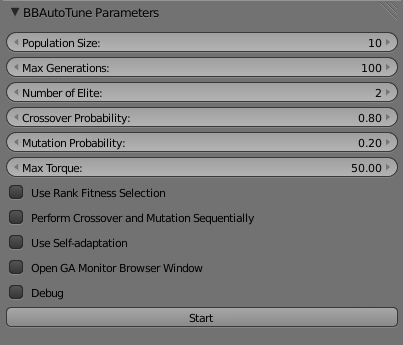
\includegraphics[scale=0.6]{../Figures/Chapter4/bbautotune_gui.png}
\rule{35em}{0.5pt}
\caption[BBAutoTune GUI Panel]{The BBAutoTune GUI panel added to Blender.}
\label{fig:bbautotune_gui}
\end{figure}

\subsection{Physics Engine API}

To provide the capability of authoring 3D interactive content, Blender uses a real-time physics engine known as Bullet. Blender exposes the Bullet physics engine API via its own Python API. Most, if not all, of the parameters to Bullet can be modified via the physics engine API during or before running the Blender game engine. Ignoring duplicate ways to set the same parameter and duplicate parameters per dimension, there are 42 different physics engine parameters that can be set via the API.

%\footnote{Bullet is the real time physics engine used by Blender. Released under the zlib license, Bullet provides real time continuous collision detection and rigid body dynamics \cite{website:continuousphysics}.}

\subsubsection{Parameter Set}

Blender's physics parameters can be set via its GUI or API. The API provides multiple avenues to set the same parameter depending on whether or not an API call is made from within Blender's built-in game engine or not. Each physics parameter is set to some default value at the start of Blender. All parameters have a range of either discrete or continuous values. Parameters such a \textit{gravity} and \textit{mass} are intended to reflect the real-world phenomena with the same names. Other parameters are more obscure such as:
\begin{enumerate}
 \item \textit{use material physics}---determines whether or not a material's physical properties (such as its friction coefficient and its collision elasticity) are taken into account during simulation;
 \item \textit{material force}---specifies an upward repellent spring like force;
 \item \textit{material damping}---dampens a material's spring force;
 \item \textit{material distance}---the distance at which a material's physical properties have an affect;
 \item \textit{material align to normal}---align physics objects along their surface normal;
 \item \textit{use actor}---determines if a physics object is seen by near and/or radar sensors;
 \item \textit{use ghost}---determines whether or not a physics object registers a collision when colliding with other physics objects;
 \item \textit{no sleeping}---if set, a physics object's position and orientation is still calculated by the physics engine even if the physics object is at rest;
 \item \textit{form factor}---the higher the value, the lower the likelihood a rigid body will roll when acted upon by some outside force;
 \item \textit{use collision bounds}---if set to false, a physics object's collision bounds is defaulted to a sphere shape;
 \item \textit{max physics steps}---specifies the maximum number of physics engine iterations per rendered frame;
 \item \textit{physics sub-steps}---specifying a higher value results in a more precise physical simulation model;
 \item \textit{FPS}---specifies the fixed physics time step such that the time step equals $\frac{1}{FPS}$ and is independent of the rendering frame rate; and
 \item \textit{deactivation time}---specifies the amount of time at which the physics engine will not longer calculate the position and orientation of a physics object that has a (angular or linear) velocity below some threshold \cite{website:blenderapi}.
\end{enumerate}
See Table \ref{tab:physics_params_ranges} for the full 41 parameter set complete with each parameter's valid range and default value.

\begin{table}[ht!]
\centering
\footnotesize
\bgroup
\def\arraystretch{1.1}
\begin{tabular}{ | >{\centering\arraybackslash}m{4cm} | >{\centering\arraybackslash}m{4cm} | >{\centering\arraybackslash}m{4cm} | }
\hline
\rowcolor{gray}
Parameter        & Range                                       & Default Value \\ \hline

Gravity          & [0.0$\frac{m}{s^2}$,10000.0$\frac{m}{s^2}$] & 9.8$\frac{m}{s^2}$ \\ \hline
Max Physics Steps & [1,5] & 5 \\ \hline
Physics Sub-steps & [1,50] & 1 \\ \hline
FPS & [1,10000] & 60 \\ \hline
Linear Deactivation Threshold & [0.001,10000.0] & 0.8 \\ \hline
Angular Deactivation Threshold & [0.001,10000.0] & 1.0 \\ \hline
Deactivation Time & [0.0s,60.0s] & 2.0s \\ \hline 

Use Material Physics & [False,True] & True \\ \hline
Material Friction & [0.0,100.0] & 0.5 \\ \hline
Material Elasticity & [0.0,1.0] & 0.0 \\ \hline
Material Force & [0.0,1.0] & 0.0 \\ \hline
Material Damping & [0.0,1.0] & 0.0 \\ \hline
Material Distance & [0.0,20.0] & 0.0 \\ \hline
Material Align to Normal & [False,True] & False \\ \hline

Physics Type & [NO\_COLLISION, STATIC, DYNAMIC, RIGID\_BODY, SOFT\_BODY, OCCLUDE, SENSOR, NAVMESH, CHARACTER] & STATIC \\ \hline
Use Actor & [False,True] & True \\ \hline
Use Ghost & [False,True] & False \\ \hline
Use Material Force Field & [False,True] & False \\ \hline
Rotate From Normal & [False,True] & False \\ \hline
No Sleeping & [False,True] & False \\ \hline
Mass             & [0.0,10000.0] & 1.0\\ \hline
Radius & [0.01m,inf] & 1m \\ \hline
Form Factor & [0.0,1.0] & 0.4 \\ \hline
Use Anisotropic Friction & [False,True] & False \\ \hline
Anisotropic Friction X,Y,Z & [0.0,1.0] & 1.0 \\ \hline
Velocity Minimum/Maximum & [0.0,1000.0] & 0.0 \\ \hline
Lock Translation X,Y,Z  & [False,True] & False \\ \hline
Lock Rotation X,Y,Z & [False,True] & False \\ \hline
Damping Translation & [0.0,1.0] & 0.025 \\ \hline
Damping Rotation & [0.0,1.0] & 0.159 \\ \hline
Use Collision Bounds & [False,True] & False \\ \hline
Collision Bounds Type & [BOX, SPHERE, CYLINDER, CONE, CONVEX\_HULL, TRIANGLE\_MESH, CAPSULE] & BOX \\ \hline
Collision Margin & [0.0m,1.0m] & 6cm \\ \hline

Force            & [-inf,inf]                                  & 0.0 \\ \hline
Torque           & [-inf,inf]                                  & 0.0 \\ \hline
Linear Velocity  & [-inf,inf]                                  & 0.0 \\ \hline
Angular Velocity & [-inf,inf]                                  & 0.0 \\ \hline
Use Local Force            & [False,True]   & True \\ \hline
Use Local Torque           & [False,True]   & True \\ \hline
Use Local Linear Velocity  & [False,True]   & True \\ \hline
Use Local Angular Velocity & [False,True]   & True \\ \hline
Damping Frames             & [-32768,32767] & 0    \\ \hline
\end{tabular}
\egroup
\caption[Blender Physics Parameters and Ranges]{The various physics parameters, their ranges, and their default values. Note that inf=340,282,346,638,528,859,811,704,183,484,516,925,440.0 in Blender.}
\label{tab:physics_params_ranges}
\end{table}

\subsection{Database Manager}

Running within Blender, the database manager opens a connection to a local MySQL database. For each evaluated genetic algorithm generation, the database manager stores the generation number, the highest fitness, the average fitness, the lowest fitness, the crossover probability, and the mutation probability in the database. 

\subsection{Robot Monitor}

Running within the Blender game engine, the robot monitor records the position and rotation state of the simulated robot's base throughout the duration of running the game engine. At the very start of the game engine, the robot monitor records the position and rotation\footnote{Position meaning its world position in the x, y, and z dimensions and rotation meaning its world orientation around the x, y, and z axes.} state $S$ of the robot's base with a time stamp $T$. After one second has passed, the robot monitor records the updated position and rotation state $S'$ of the robot's base with a time stamp $T'$. At this point, if the robot's base has come to a rest, the robot monitor exits the game engine. Otherwise, if the robot's base is still moving, the robot monitor will update $S'$ and $T'$ every half second for the rest of the evaluation period. After 16 seconds have elapsed, the robot monitor exits the game engine regardless of whether or not the robot's base is still moving. Every time the robot monitor records $S'$ and $T'$, it writes $S$, $T$, $S'$, and $T'$ to a file that will be later read by the fitness function.  

\subsection{Progress Monitor}

The progress monitor is an external and self-contained Python HTTP-CGI server that listens on port 8000. By visiting  \texttt{http://localhost:8000/index.py}, a user can track the GA's progress concerning the highest fitness, average fitness, lowest fitness, crossover probability, and the mutation probability. See Figure \ref{fig:ga_monitor}. Once the user presses start on the GUI panel, BBAutoTune starts the server as an external process with the option of opening a browser to the progress page. Once every minute, the progress monitor retrieves the most current GA run information from the local MySQL database which was populated by the database manager.

\begin{figure}[ht!]
\centering
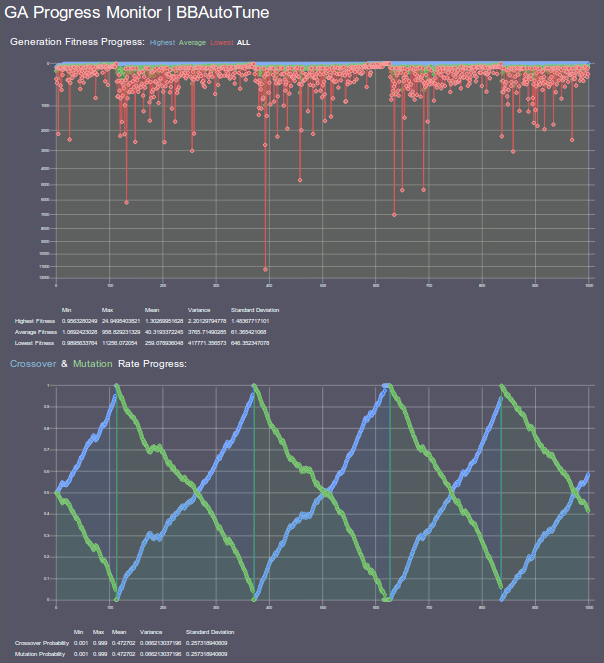
\includegraphics[scale=0.6]{../Figures/Chapter4/ga_monitor.png}
\rule{35em}{0.5pt}
\caption[GA Progress Monitor]{The external GA progress monitor.}
\label{fig:ga_monitor}
\end{figure}

\subsection{Genetic Algorithm}

The genetic algorithm for BBAutoTune was borrowed from the SimPL project and ported to Python with some aspects of the GA being altered to suit the needs of BBAutoTune. Since lower values of fitness are considered beter than those of higher values of fitness, the population sorting function needed to be altered. Other portions altered were the selection operator, the population metrics calculator, and the self-adaptation algorithm.  

\subsubsection{Encoding Scheme}

The physics parameters selected for tuning were a mixed set of floats, integers, string arrays, and boolean values (see Table \ref{tab:physics_params_ranges}). To ease the process of crossover and mutation, all genome genes were homogenized to a normalized range of $[0.0,1.0]$. Let any given genome's gene value be $g_i$ and any given physics parameter be $p_i$. For a float type with a maximum range value $r_{max}$ and minimum range value $r_{min}$, the decoding function was $p_i=(g_i*(r_{max}-r_{min}))+r_{min}$. For an integer type, the decoding function was the same as for a float type except the whole value was floored. For an array $A$ of strings type with size $n$ (for example the collision bounds type parameter), the decoding function was $p_i=A[\lfloor g_i*(n-1)\rfloor]$. Finally for a boolean type, the decoding function was 

\[ p_i = \left\{
\begin{array}{l l}
True & \quad \text{if $g_i\geq 0.5$,}\\
False & \quad \text{if $g_i < 0.5$.}
\end{array} 
\right.\]

\subsubsection{Operators}

The operators used include selection, elitism, crossover, and mutation. All of these operators work together to generate a new population once the current population has been fully evaluated by the fitness function.

The selection operator includes two variants: tournament selection and rank fitness selection. The user can indicate on the GUI panel if rank fitness selection is to be used---otherwise tournament selection will be used. Tournament selection works by gathering a sub-portion of the total population where the fittest genome among the sub-portion is selected thereby winning the tournament \cite{Miller95geneticalgorithms}. While gathering the sub-portion, all genomes in the population have a uniform probability of being included in the tournament, regardless of their respective fitness values. There is the possibility that the same genome may be included in the tournament more than once. For crossover, two tournaments of size three are run, thereby giving two genomes to be crossed. For mutation, one tournament of size two is run, thereby giving one genome to be mutated. Rank fitness selection works by first sorting the population in non-increasing order according to fitness and then selects a genome at random where the probability of a genome being selected is proportional to its rank fitness. With the population in sorted order, the first genome is given a rank fitness of 1, the second genome is given a rank fitness of 2, ..., and the last genome is given a rank fitness of $n$ which is the population size. The rank fitness prefix-sum for each genome is calculated in an array such that the first index value in the prefix-sum array is $1$ while the last index value in the prefix-sum array is $\frac{n(n-1)}{2}$. A uniform random number is selected in the range $\left[0,\frac{n(n-1)}{2}\right]$. The genome selected $G$ is the one in which the random number is greater than the previous prefix-sum for genome $G_{i-1}$ and less than or equal to the prefix-sum for $G_i$. Genomes with a higher fitness will have a higher rank fitness and thus will have a higher probability of being selected for either crossover or mutation. See Figures \ref{fig:rank_fitness_selection} and \ref{fig:rank_fit_example}. 

\renewcommand{\baselinestretch}{1.0}

\begin{figure}[htbp]
\begin{center}
\begin{varwidth}{\textwidth}
{\tt
BEGIN \\
\tab Population $P$ with size $n$ has been evaluated \\
\tab Sort $P$ in non-increasing order \\
\tab For i=1 to $n$ do \\
\tab \tab $P[i-1].rankFitness = i$ \\
\tab End for \\
\tab For i=0 to $n-1$ do \\
\tab \tab $P[i].prefixSum = \sum\limits_{k=0}^i(P[k].rankFitness)$ \\
\tab End for \\
\tab Select a random number $r=unif\left(0,\frac{n(n-1)}{2}\right)$ \\
\tab Genome selected $G$ \\
\tab For i=0 to $n-1$ do \\
\tab \tab If $P[i].prefixSum \geq r $ then \\
\tab \tab \tab $G=P[i]$ \\
\tab \tab \tab Break \\
\tab \tab End if \\
\tab End for \\
\tab Return $G$ \\
END \\
}
\end{varwidth}
\end{center}
\centering
\rule{35em}{0.5pt}
\caption[Rank Fitness Selection Algorithm]{The rank fitness selection algorithm.}
\label{fig:rank_fitness_selection}
\end{figure}

\begin{figure}[ht!]
\centering
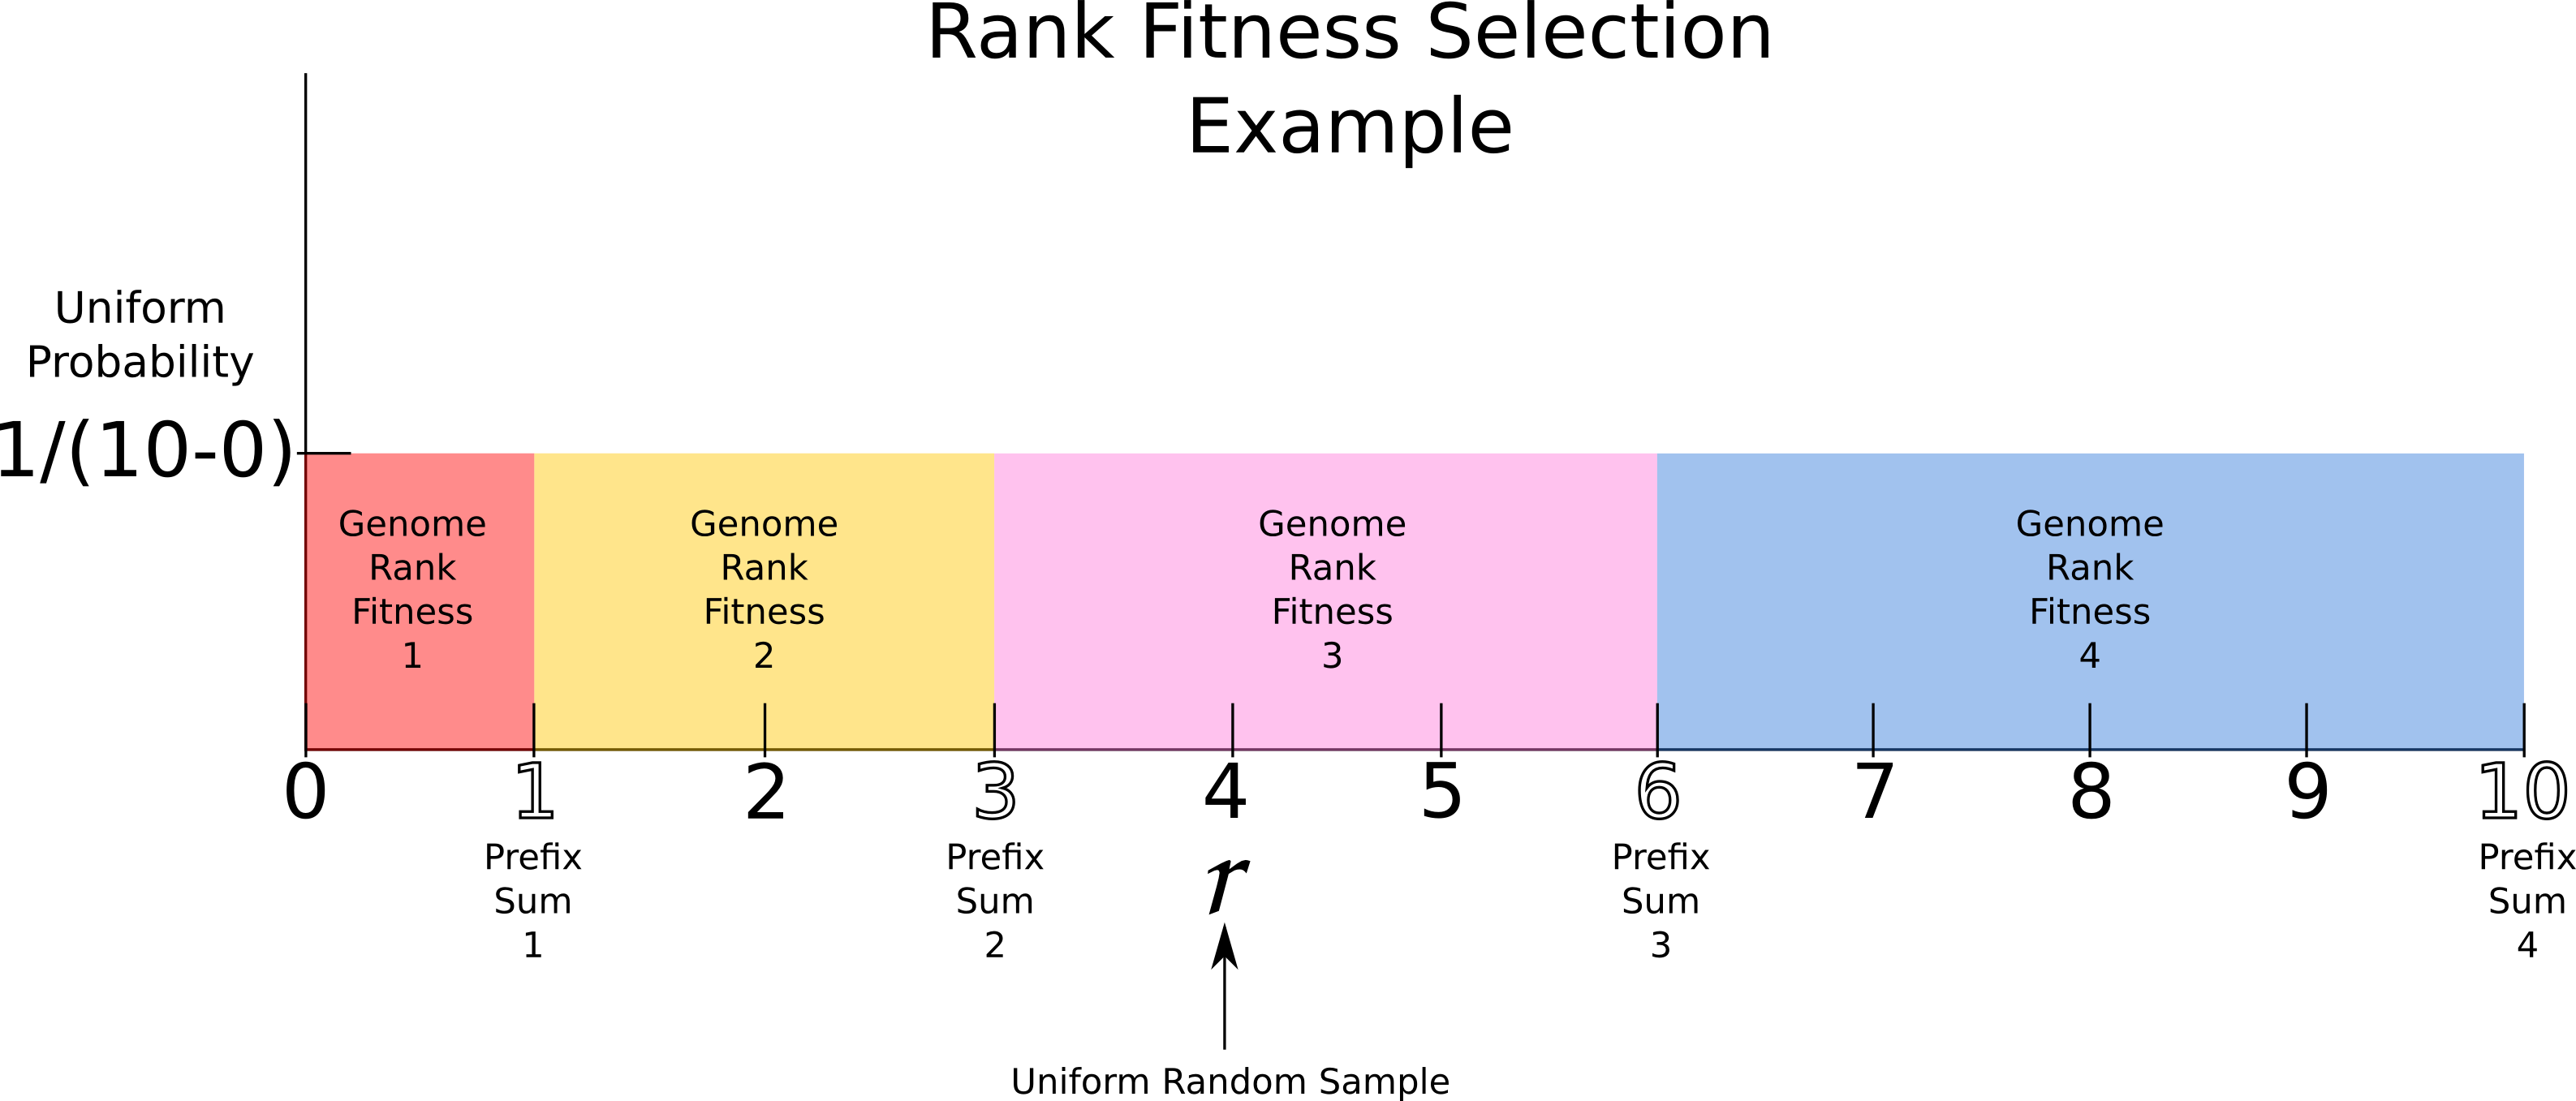
\includegraphics[scale=0.6]{../Figures/Chapter4/rank_fit_example.png}
\rule{35em}{0.5pt}
\caption[Rank Fitness Selection Illustration]{An illustrative rank fitness selection example. The population consists of four genomes where the rank fitnesses are one, two, three, and four. The prefix-sums are one, three, six, and 10. A random integer is sampled from a uniform distribution between zero and 10. Since the random number was four, the genome with a rank fitness of 3 would be selected. Notice that genomes with a higher rank fitness, have a greater uniform probability of being selected.}
\label{fig:rank_fit_example}
\end{figure}

\subsubsection{Fitness Function}

%\todo{This section only reflects the data recorded using the old move() function. Change to reflect data collected using the new motion() function.}

To construct the fitness function, real robot motion data was collected which included 1040 sample points. Each sample point consisted of the x-position, y-position, and heading (z-orientation) of the robot before it moved and the x-position, y-position, and heading after the robot moved. With a camera overhead, the real robot was placed in the arena and was repeatedly commanded to go forward (relative from its current position and orientation) 25 centimeters. Care was taken to avoid having the robot collide with the arena walls. Once the robot consecutively moved forward three times, the robot rotated in place by 135 degrees and was not recorded during this period of rotation.  

Using the camera, the robot's position and orientation before and after performing each forward command was recorded. The robot's position and orientation were not reset each time the robot performed a forward command. Instead, the robot was allowed to continue forward from its current position and orientation as it traveled around the arena. Thus each recorded pair of initial and final states was translated and rotated to be in the same reference frame such that the robot was always at the arena origin facing down the global positive x-axis before performing the forward command. See Figures \ref{fig:real_robot_raw_trans_rot} and \ref{fig:real_robot_forward_motion}. Note that from the robot's perspective, it is always facing down its local positive x-axis no matter its position or orientation as seen from some other reference point. With all of the data transformed and rotated, each initial state had a x-position of 0.0, a y-position of 0.0, and an initial orientation of 0.0 degrees. 

\begin{figure}[htbp]
\centering
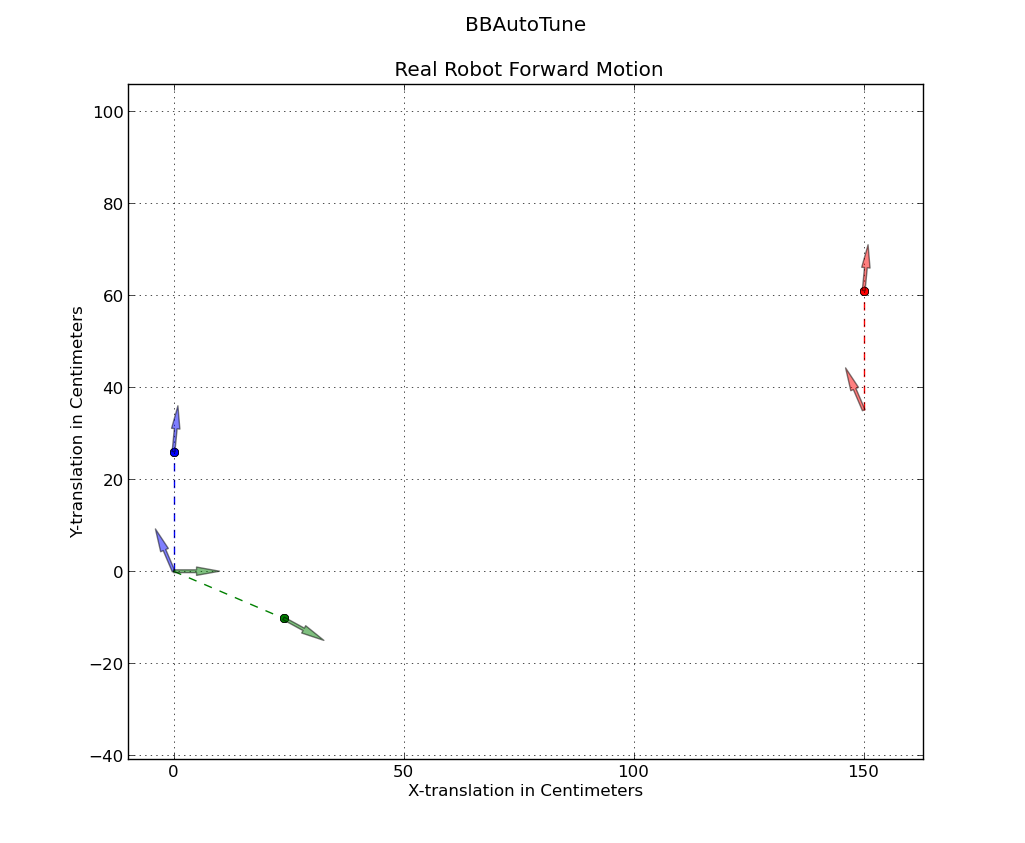
\includegraphics[scale=0.6]{../Figures/Chapter4/real_robot_raw_trans_rot.png}
\rule{35em}{0.5pt}
\caption[Real Robot Forward Motion Data Translated and Rotated Example]{A specific instance of how the raw real robot forward motion data was translated and rotated such that each pair of initial and final states have the same reference frame. The red arrows, dot, and line represent the raw initial and final state of the robot recorded from the overhead camera before and after it performed the forward command. The blue arrows, dot, and line represent the initial and final state translated to the origin. The green arrows, dot, and line represent the initial and final state rotated by the amount needed to align the initial orientation with the positive global x-axis. For each colored group, the dot and arrow pair represent the position and orientation of the robot after having performed the forward command, while the arrow without a dot represents the position and orientation state of the robot before it performed the forward command.}
\label{fig:real_robot_raw_trans_rot}
\end{figure}

\begin{figure}[htbp]
\centering
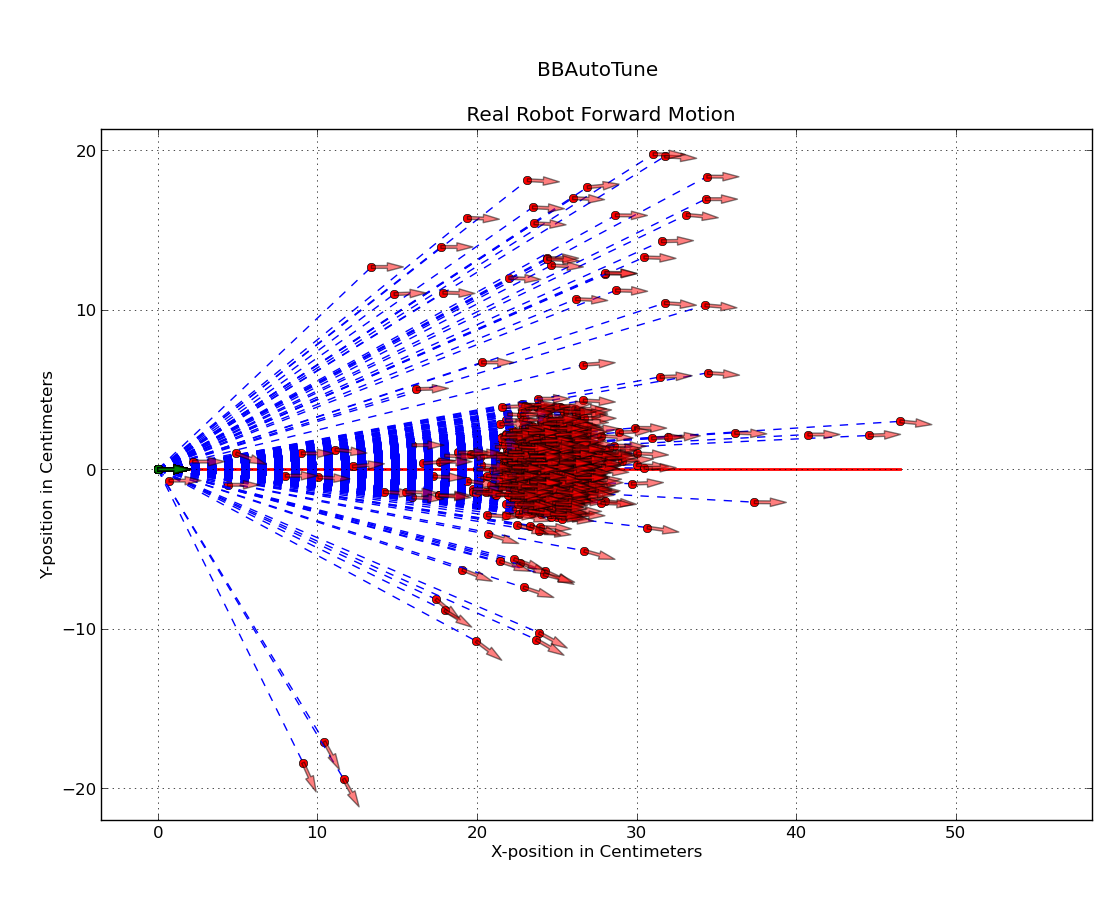
\includegraphics[scale=0.6]{../Figures/Chapter4/real_robot_forward_motion.png}
\rule{35em}{0.5pt}
\caption[Real Robot Forward Motion]{The collected real robot forward motion plotted from the same reference point. The green dots and arrows indicate the starting position and orientation of the real robot before the forward command was performed. The red dots and arrows indicate the ending position and orientation of the real robot after the forward command was performed. The dots represent position and the arrows represent orientation. The broken blue lines connect the initial states to their corresponding finals states.}
\label{fig:real_robot_forward_motion}
\end{figure}

Analyzing the distribution of final state x-positions, y-positions, and headings separately, all are unimodal and nearly symmetric with only a slight skew from their respective means. See Table \ref{tab:real_robot_motion_dist} and Figure \ref{fig:real_robot_forward_dist}. When viewing the dimensions together, a large mass is centered around the point: 23.8644631679cm, 0.338269853117cm, and -0.00417473025048rad. See Figure \ref{fig:real_robot_3d_scatter}. Based on the variance-covariance matrix, all three dimensions vary together and are not independent of one another.

\begin{table}[htbp]
\centering
\footnotesize
\bgroup
\def\arraystretch{1.1}
\begin{tabular}{ | >{\centering\arraybackslash}m{3cm} | >{\centering\arraybackslash}m{3cm} | >{\centering\arraybackslash}m{3cm} | >{\centering\arraybackslash}m{3cm} | }
%\hline
%\rowcolor{gray}
\cline{2-4}
\multicolumn{1}{c|}{}                  & \cellcolor{gray} X-position & \cellcolor{gray} Y-position & \cellcolor{gray} Heading \\ \hline
\cellcolor{gray} Maximum                  & 46.5183415482cm        & 19.7486813209cm       & 6.23776rad           \\ \hline
\cellcolor{gray} Minimum                  & 0.0cm                  & -19.4028539247cm      & -1.148163rad         \\ \hline
\cellcolor{gray} Mean/Centroid         & 23.8644631679cm        & 0.338269853117cm      & -0.00417473025048rad \\ \hline
\cellcolor{gray} Mode                  & 25.0cm                 & -1.0cm                & 0.0rad               \\ \hline
\cellcolor{gray} Variance              & 10.3960320996          & 9.46441502772         & 0.152467827567       \\ \hline
\cellcolor{gray} Standard Deviation    & 3.22428784378          & 3.07642894079         & 0.390471289043       \\ \hline
\cellcolor{gray} Covariance with X-position  & 10.4060572             & 2.3348963             & 0.0685591            \\ \hline
\cellcolor{gray} Covariance with Y-position  & 2.3348963              & 9.47354175            & 0.08654865           \\ \hline
\cellcolor{gray} Covariance with Heading     & 0.0685591              & 0.08654865            & 0.15261486           \\ \hline
\end{tabular}
\egroup
\caption[Real Robot Forward Motion Distribution Metrics]{The distribution metrics of final state x-positions, y-positions, and headings after the real robot moved forward.}
\label{tab:real_robot_motion_dist}
\end{table}

% Number of sample points:  1040
% X' max/min:  46.5183415482 0.0
% X' mode:  (array([ 25.]), array([ 8.]))
% X' mean:  23.8644631679
% X' variance:  10.3960320996
% X' standard deviation:  3.22428784378
% Y' max/min:  19.7486813209 -19.4028539247
% Y' mode:  (array([-1.]), array([ 8.]))
% Y' mean:  0.338269853117
% Y' variance:  9.46441502772
% Y' standard deviation:  3.07642894079
% Theta' max/min:  6.23776 -1.148163
% Theta' mode:  (array([ 0.]), array([ 234.]))
% Theta' mean:  -0.00417473025048
% Theta' variance:  0.152467827567
% Theta' standard deviation:  0.390471289043
% X' normal test p-value:  2.45603600615e-124 Not Normal
% Y' normal test p-value:  1.60589004385e-121 Not Normal
% T' normal test p-value:  0.0 Not Normal
% Covariance matrix: 
% [[ 10.4060572    2.3348963    0.0685591 ]
%  [  2.3348963    9.47354175   0.08654865]
%  [  0.0685591    0.08654865   0.15261486]]
% X', Y', T' Median:  24.0201969119 ,  0.0475373929135 ,  -0.0145985
% X'Y'T' Centroid:  23.8644631679 ,  0.338269853117 ,  -0.00417473025048
% X'Y'T' Geometric Median:  23.9754618867 ,  0.0401244563225 ,  -0.0124671288475

\begin{figure}[htbp]
\centering
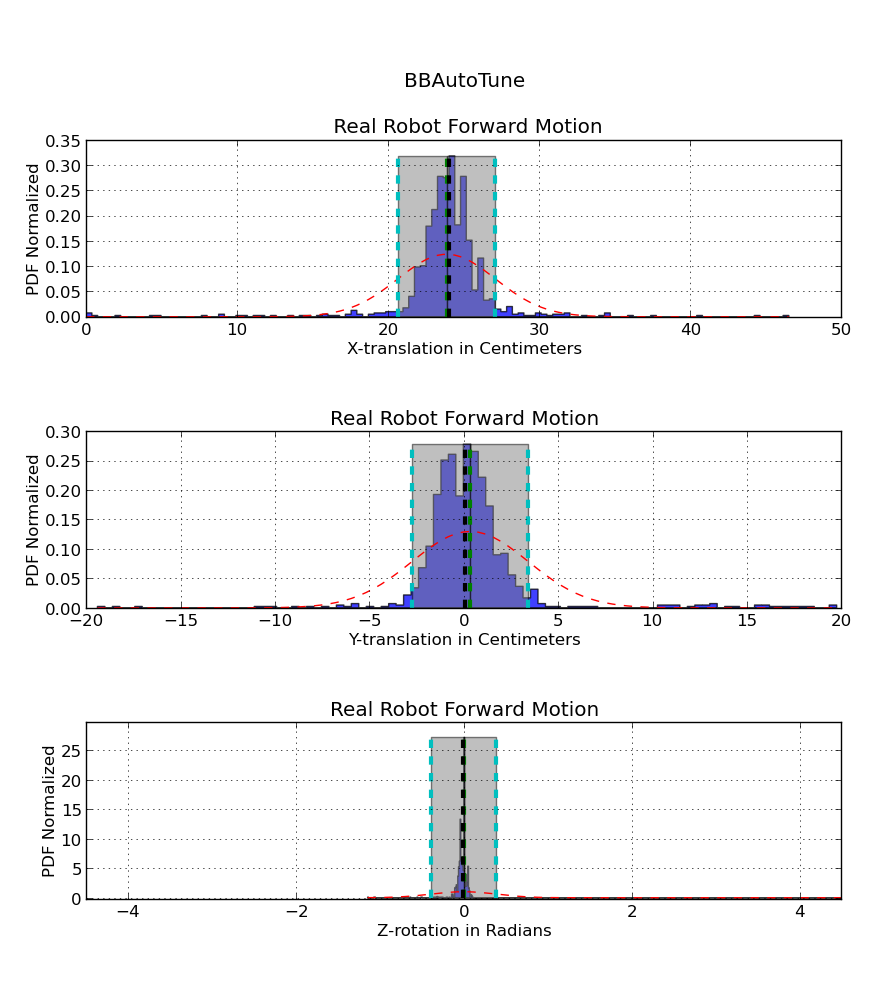
\includegraphics[width=5.5in]{../Figures/Chapter4/real_robot_forward_dist.png}
\rule{35em}{0.5pt}
\caption[Real Robot Forward Motion Distributions]{The distributions of final state x-positions, y-positions, and headings (after being translated and rotated to the same reference frame) recorded for the real robot forward motion. The broken black bar represents the mode, the green broken bar represents the mean, the cyan broken bars represent one standard deviation from the mean, and the red broken curve represents the best fit normal curve.}
\label{fig:real_robot_forward_dist}
\end{figure}

\begin{figure}[htbp]
\centering
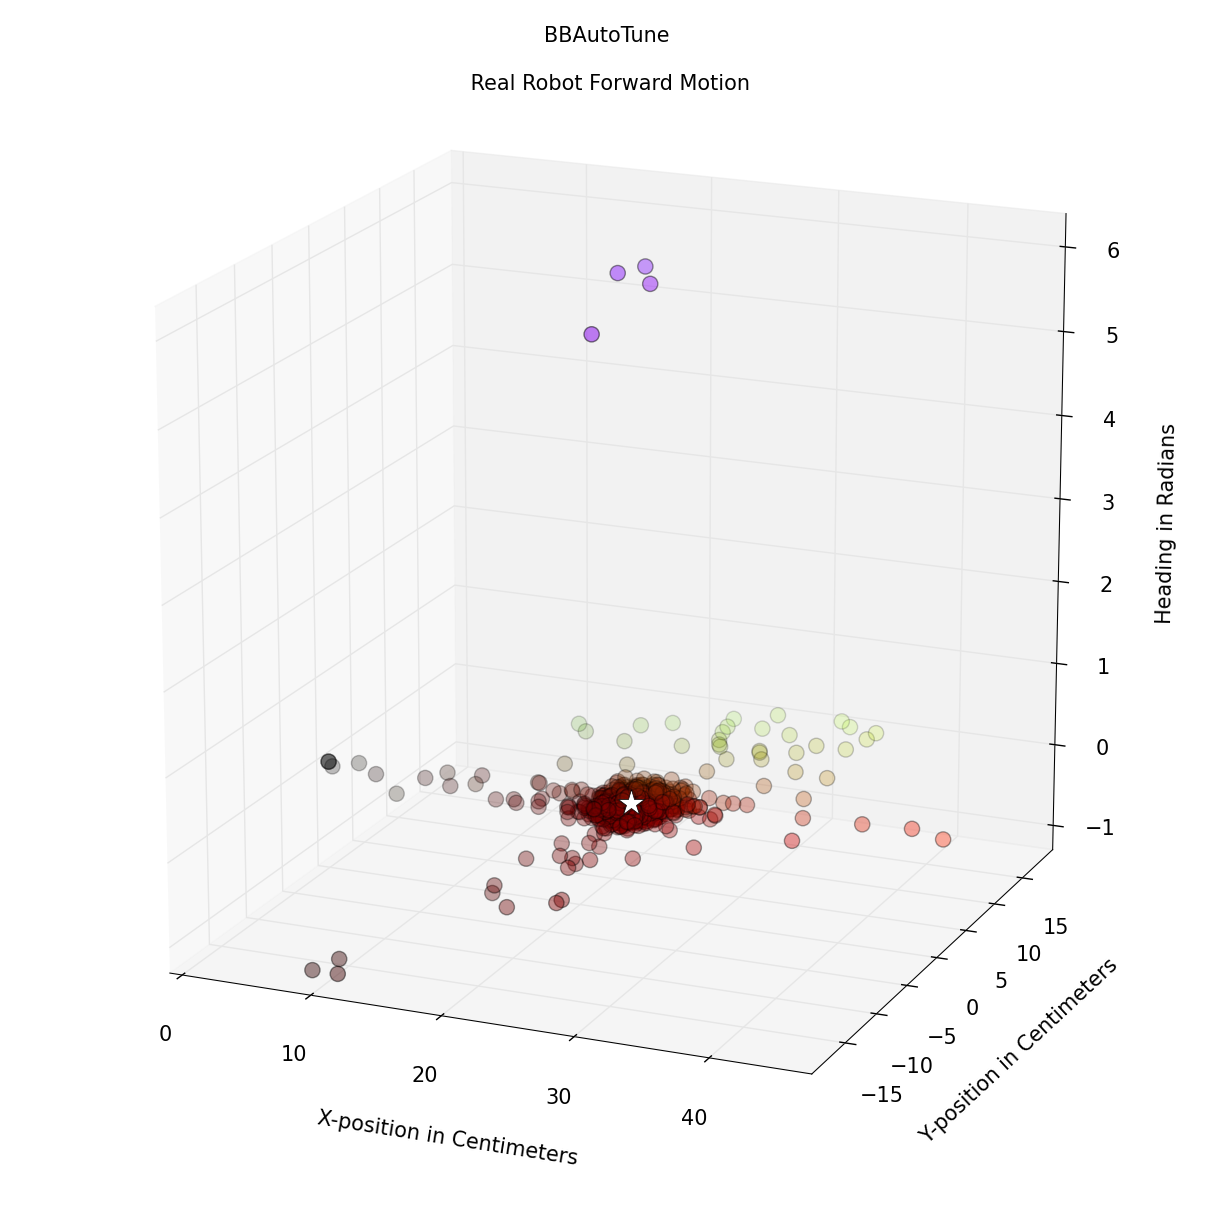
\includegraphics[scale=0.5]{../Figures/Chapter4/real_robot_3d_scatter.png}
\rule{35em}{0.5pt}
\caption[Real Robot Forward Motion 3D Scatter Plot]{A 3D scatter plot of final state x-positions, y-positions, and heading values for the real robot after it performed the forward command. Positive values of x-position, y-position, and heading contribute a portion of red, green, and blue respectively to each scatter plot. The star located at the center of the large mass of points is the centroid.}
\label{fig:real_robot_3d_scatter}
\end{figure}

With the real robot motion data collected and analyzed, a metric was needed for the fitness function. This metric would need to indicate how different or dissimilar the movement of the simulated robot was from the real robot while running the GA. The intuition was that as the simulated robot motion moved closer to the centroid of the real robot motion, the simulated motion would become increasingly indistinguishable from the real motion. Various distance functions were considered and the Mahalanobis distance (MD) was chosen as the basis for the fitness function. The MD is a generalized form of the Euclidean distance, such that the MD accounts for the correlation in the data set since it is computed using the inverse of the variance-covariance matrix \cite{mahalanobis_distance}. For uncorrelated data, the MD reduces to the Euclidean distance \cite{what_is_mahalanobis_distance}.

Noise introduced by the overhead camera and the timing at which the position and orientation state of the real robot was captured could have potentially skewed the real robot motion model with outliers, ultimately resulting in a skewed multivariate mean location and a skewed inverse variance-covariance matrix, making the MD skewed. To account for the potential outliers in the real motion data set, a robust\footnote{\textit{Robust} meaning the robustness of an estimator's resistance to outliers or data point contamination \cite{WICS:WICS61}.} mean location and a robust variance-covariance matrix was computed from the data set using the Fast-MCD algorithm implemented in the Scikit-learn Python module \cite{Rousseeuw:1999:FAM:331435.331458}\cite{scikit-learn}. The classical mean location was 23.8644632cm, 0.338269853cm, and -0.00417473025rad for final state x-positions, y-positions, and headings respectively while the robust mean location was 23.9934044cm, 0.0351240536cm, and -0.0189964938rad for final state x-positions, y-positions, and headings respectively. The left matrix below is the classical variance-covariance matrix, while on the right is the robust variance-covariance matrix returned by the Fast-MCD algorithm.
\vspace{-1mm}
\[ \left( \begin{array}{ccc}
10.3960321 &  2.33264688 & 0.06849305 \\
2.33264688 &  9.46441503 & 0.08646527 \\
0.06849305 &  0.08646527 & 0.15246783 \\
\end{array} \right)
%
\left( \begin{array}{ccc}
1.46298445 & 0.13924542 & 0.00223493 \\
0.13924542 & 1.64197605 & 0.0168499  \\
0.00223493 & 0.0168499  & 0.00173777 \\
\end{array} \right)
\]

\noindent
The resulting samples weighted higher than others by the Fast-MCD algorithm are shown in Figure \ref{fig:robust_support_samples}. These samples were used to calculate the robust mean and the robust variance-covariance matrix returned by the algorithm. By substituting the robust mean and the inverse of the robust variance-covariance matrix into the MD calculation, the robust distance (RD) for any sample point can be computed \cite{WICS:WICS61}. Comparisons between the MD and the RD for each of the 1040 real robot motion data points are shown in Figure \ref{fig:real_robot_md_vs_rd}. As the data points travel away from the centroid, the RD increases more rapidly than the MD.  

% Classical Mean (Location):  [  2.38644632e+01   3.38269853e-01  -4.17473025e-03]
% Robust Mean (Location):  [  2.39934044e+01   3.51240536e-02  -1.89964938e-02]
% Classical Covariance Matrix: 
% [[ 10.3960321    2.33264688   0.06849305]
%  [  2.33264688   9.46441503   0.08646527]
%  [  0.06849305   0.08646527   0.15246783]]
% Robust Covariance Matrix: 
% [[ 1.46298445  0.13924542  0.00223493]
%  [ 0.13924542  1.64197605  0.0168499 ]
%  [ 0.00223493  0.0168499   0.00173777]]   

\begin{figure}[htbp]
\centering
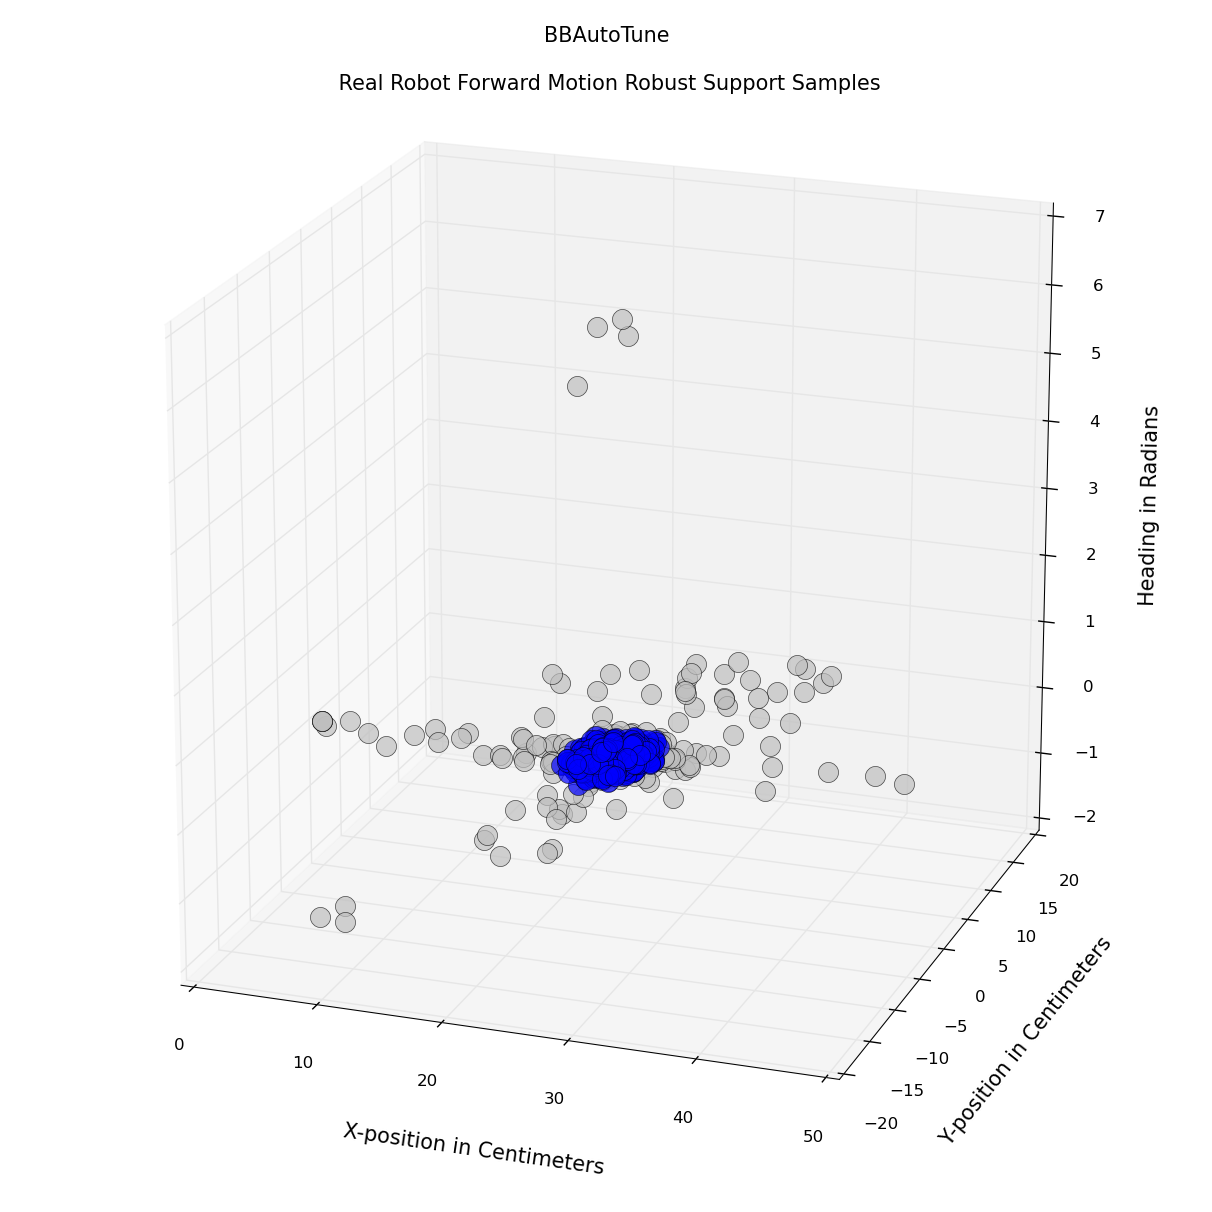
\includegraphics[scale=0.5]{../Figures/Chapter4/real_robot_robust_samples.png}
\rule{35em}{0.5pt}
\caption[Real Robot Forward Motion Fast-MCD Support Samples]{A 3D scatter plot of the support samples in blue used to calculate the robust mean location and the robust variance-covariance matrix as returned by the Fast-MCD algorithm.}
\label{fig:robust_support_samples}
\end{figure}

\begin{figure}[htbp]
\centering
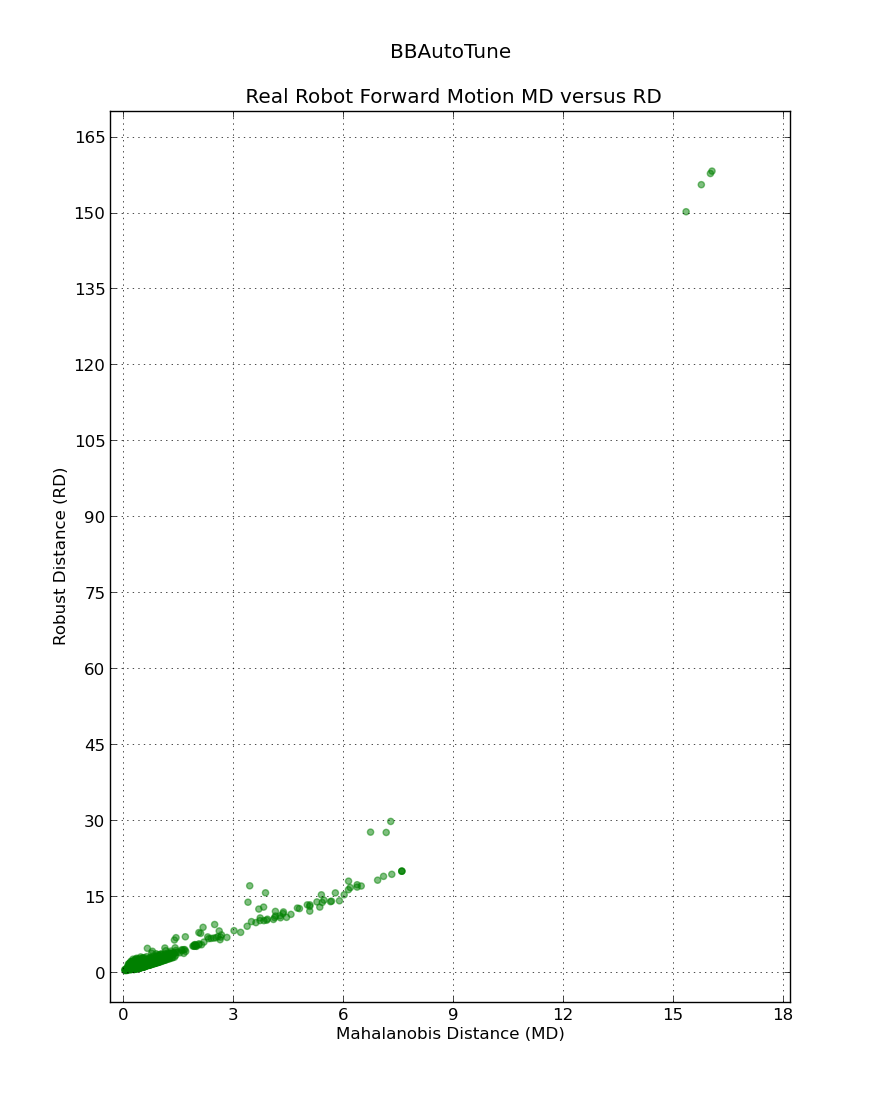
\includegraphics[height=8in]{../Figures/Chapter4/real_robot_md_vs_rd.png}
\rule{35em}{0.5pt}
\caption[Real Robot Forward Motion MD versus RD]{A scatter plot comparing the Mahalanobis distance versus the robust distance for each data point collected of the real robot motion.}
\label{fig:real_robot_md_vs_rd}
\end{figure}

Only three out of the total six degrees of freedom were recorded for the real robot. However, in Blender there were an additional three degrees of freedom (pitch, roll, and heave or up and down) to contend with. Thus, the simulated-robot base's x-rotation, y-rotation, and z-translation were constrained. Additionally, all wheels had their z-translation constrained. As an added precaution, penalties were added onto the robust distance by the absolute amount the simulated robot's base violated any rotation around the global x-axis, any rotation around the global y-axis, and/or any translation up or down the global z-axis. Additionally, a time penalty was added onto the robust distance by the amount of time in seconds the simulated robot took to evaluate (or rather took to come to a complete stop) greater than one second with a maximum penalty of 15 seconds since any given evaluation period only lasted a total of 16 seconds. This time penalty was necessary since it was observed that the real robot never took more than one second to come to a complete stop after moving forward. Without a time penalty, for example, a simulated robot could move just as the real robot and it would be given an erroneously high fitness even though it took 16 seconds to come to a complete stop. This undesirable scenario was avoided by using a time penalty.     

Once the simulated robot was run through the game engine evaluation period (using the physics parameter settings decoded from the currently being evaluated genome $G_i$'s genes), 14 pieces of data was collected by the robot monitor for use in the fitness function. Let $S=[x_p,y_p,z_p,x_o,y_o,z_o,T]$ be the starting state of the simulated robot at the beginning of the evaluation period at time $S[6]=T$ where the subscript $_p$ refers to position and the subscript $_o$ refers to orientation. Let $S'=[x_p,y_p,z_p,x_o,y_o,z_o,T']$ be the ending state of the simulated robot at the end of the evaluation period at time $S'[6]=T'$. Also, let $RD(x-position,y-position,z-orientation)$ be the robust distance. The fitness of $G_i$ was defined as $Fitness(S,S')=RD(S'[0],S'[1],S'[5])+|S'[4]-S[4]|+|S'[3]-S[3]|+|S'[2]-S[2]|+((S'[6]-S[6])-1)=G_i$'s fitness. The range of this function is $[0,\infty)$. Since the goal of this thesis was to have the simulated robot move as the real robot, the desired output of this function was $0.0$ implying that three objectives were met:
\begin{itemize}
 \item The simulated robot's x-position, y-position, and z-orientation (heading) after moving forward was 23.9934044cm, 0.0351240536cm, and -0.0189964938rad respectively.
 \item The simulated robot came to a complete stop after one second.
 \item The simulated robot did not fall through the floor, flip over, roll over, and/or launch upward.
\end{itemize}
Thus the goal of the GA was to minimize this function whereby lower output values were a higher fitness than higher output values.

\subsubsection{Evaluation Setup}

For each evaluation period (the running of the game engine), the 3D robot model's local coordinate system was axis aligned with the world coordinate system, the robot was faced forward looking down the positive global x-axis, and its local origin was placed at the world origin. See Figure \ref{fig:simu_robot_aligned}. Before each evaluation period, the physics engine parameters were set to the values decoded from the genes of the currently being evaluated genome. All evaluation periods lasted no more than 16 seconds. If the robot stopped moving before 16 seconds, then the evaluation period ended immediately. The only applied force to the robot was the wheel torque, where each wheel received the same amount of applied torque for the same duration. The duration of applied torque was roughly 16 milliseconds after which no further force was applied to the robot.

\begin{figure}[htbp]
\centering
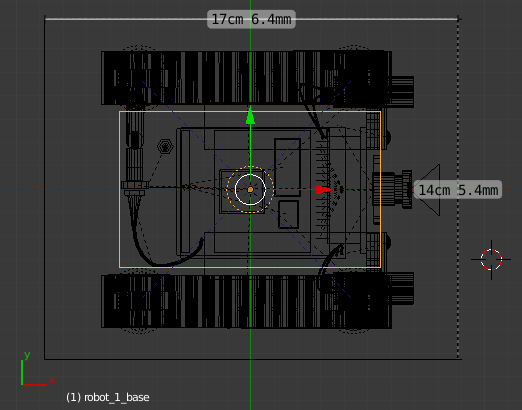
\includegraphics[scale=0.5]{../Figures/Chapter4/simu_robot_aligned.png}
\rule{35em}{0.5pt}
\caption[Simulated Robot Axis Aligned]{The simulated robot's local coordinate system axis aligned with the world coordinate system.}
\label{fig:simu_robot_aligned}
\end{figure}

\section{Platform}

For all experiments, BBAutoTune was run on a 64bit Linux operating system with 32GB of RAM and an Intel Core i7-4770K four core processor running at 3.9GHz.

\section{Experimental Designs}

The purpose for experiment one was to determine a base set of physics parameters that have significant influence over the physics simulation. Experiments two through five involved actually tuning the physics engine and comparing the simulated versus real robot motion. Self-adaptation and tournament versus rank fitness selection were the experimental GA parameters for experiments two through five. 

\subsection[Experiment One]{Experiment one: physics engine parameter influence.}

The potential Blender physics engine parameter candidates---to be tuned by the GA---were analyzed for their influence over the physics simulation. To accomplish this goal, a racquetball-like environment was constructed in Blender which consisted of a ball, an enclosed arena, and an automated racquet controlled via a Python script. See Figure \ref{fig:racquetball}. Note that the ball was allowed to travel in all three dimensions and was completely physics based.

\begin{figure}[htbp]
\centering
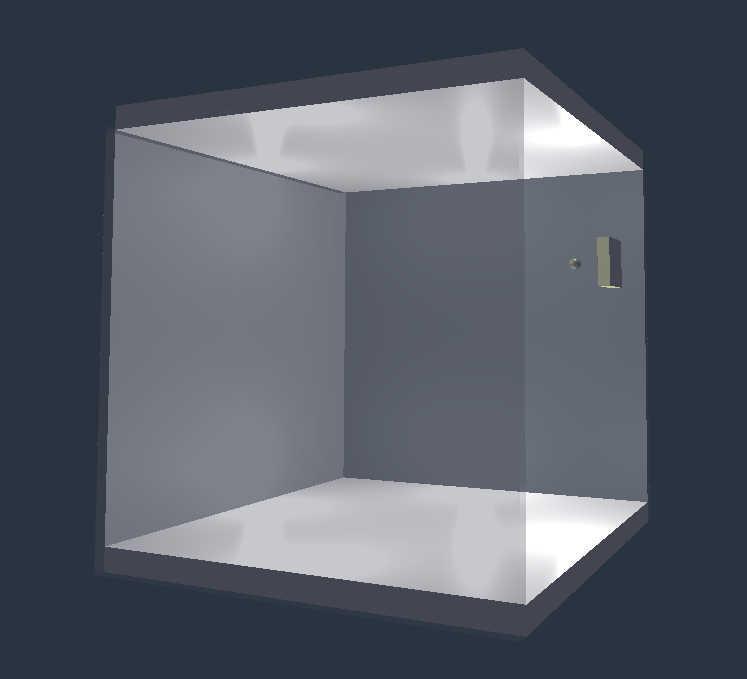
\includegraphics[scale=0.4]{../Figures/Chapter4/racquetball.png}
\rule{35em}{0.5pt}
\caption[Physics Engine Parameter Influence Racquetball Environment]{The racquetball environment used to test the physics engine parameter candidates' influence over the physics simulation.}
\label{fig:racquetball}
\end{figure}

Fourty-four candidate parameters were selected for testing in the racquetball environment (see Table \ref{tab:distances}). All parameters tested were only associated with the ball. Before all of these parameters were tested for their influence, \textit{nice} values were selected for each such that the ball's behavior appeared normal based on visual observation. A standard was established where the ball was allowed to run for five seconds (with all parameters being set to their nice values) during which its location was recorded at roughly 60 times per second. With the standard established---with which all other runs would be compared to---a parameter was selected (from the candidate pool), its value was tweaked, the ball was run for five seconds with its location being recorded at roughly 60 times per second, and after the run was over, the tweaked parameter's value was set back to its nice value. This sequence was repeated for all 44 candidate parameters.

\subsection[Experiment Two]{Experiment two: tournament selection with self-adaptation.}

Very early runs of BBAutoTune attempted to tune physics parameters: gravity, sub-steps, FPS, use material physics, material friction, material elasticity, mass, form factor, velocity maximum, damping translation, damping rotation, use collision bounds, collision bounds type, and torque, where the search space for each parameter was its entire valid range. This proved to be problematic since some of the valid ranges are quite large, especially torque with a maximum upper bound of $~3.40\times10^{38}$. While running the game engine, if the genome's genes decoded to relatively high physics engine parameter values, world coordinates would return the Python values ``NaN'' or ``inf''.

To rectify this issue, the set of physics parameters selected for tuning was pruned and for the parameters left, their ranges were shortened to reasonable upper and lower bounds found manually. The resulting set of tunable physics parameters and their ranges for experiment two were: gravity [0.0,15.0], sub-steps [1,5], FPS [30,10000], material friction [0.0,100.0], material elasticity [0.0,1.0], mass [0.010,15.0], velocity maximum [0.0,1000.0], damping translation [0.0,1.0], damping rotation [0.0,1.0], collision bounds type [TRIANGLE\_MESH,CONVEX\_HULL,CYLINDER,SPHERE], and torque [0.0,100.0]. Use material physics and use collision bounds were set to true and held constant. Form factor was set to 1.0 and was held constant. 

The GA was run for 500 generations, tournament selection was used, the population size was set to 10, elitism was set to 2, crossover and mutation were performed separately, and the crossover and mutation probabilities were self-adapted over time.

\subsection[Experiment Three through Five]{Experiment three through five.}

Experiments three through five had the exact same setup as experiment two, except for the selection method and whether or not self-adaptation was used. Experiment three used tournament selection without self-adaptation. Experiment four used rank fitness selection with self-adaptation. Lastly, experiment five used rank fitness selection without self-adaptation. 

% \subsection[Experiment Three]{Experiment three: tournament selection without self-adaptation.}
% 
% The set of tunable physics parameters for experiment three was the same as experiment two. The GA was run for 500 generations, tournament selection was used, the population size was set to 10, elitism was set to 2, crossover and mutation were performed separately, and the crossover and mutation probabilities were held constant at 0.8 and 0.2 respectively.
% 
% \subsection[Experiment Four]{Experiment four: rank fitness selection with self-adaptation.}
% 
% The set of tunable physics parameters for experiment four was the same as experiment two. The GA was run for 500 generations, rank fitness selection was used, the population size was set to 10, elitism was set to 2, crossover and mutation were performed separately, and the crossover and mutation probabilities were self-adapted over time.
% 
% \subsection[Experiment Five]{Experiment five: rank fitness selection without self-adaptation.}
% 
% The set of tunable physics parameters for experiment five was the same as experiment two. The GA was run for 500 generations, rank fitness selection was used, the population size was set to 10, elitism was set to 2, crossover and mutation were performed separately, and the crossover and mutation probabilities were held constant at 0.8 and 0.2 respectively.

\section{Experimental Results}

Experiment two had the highest performing genome out of experiments two through five. Experiments three through five had similar highest fitnesses. Using self-adaptation with tournament selection resulted in the highest fitness observed among experiments two through five. Comparing experiment two to three, self-adaptation was beneficial, but was not beneficial when comparing experiment five to four.   

\subsection[Experiment One]{Experiment one: physics engine parameter influence.}

To compare the recorded tweaked-parameter ball paths with the recorded standard, four methods were utilized to give an indication as to how much influence any one candidate parameter had over the simulation. The first method was visual inspection. All 44 tweaked-parameter ball paths were plotted against the standard. See Figure \ref{fig:matphysplot} and Figure \ref{fig:logicstepsplot}. The second method was an algorithm developed by the author, titled the \textit{Lettier distance}, which gives the maximum Euclidean distance between two discrete curves $P$ and $Q$. Informally, imagine holding a rubber band in your hands where the left hand affixes the left end of the rubber band to the first point in $P$ and the right hand affixes the right end of the rubber band to the first point in $Q$. During each iteration, you advance the left end of the rubber band to the next point in $P$ and you advance the right end of the rubber band to the next point in $Q$. If the distance grows between point $p_i\in P$ and point $q_j \in Q$, the rubber band stretches but never shrinks. If $|P|<|Q|$ then you hold the left end of the rubber band to the last point in $P$ and continue advancing to the last point in $Q$ and vice versa. Once you reach the last point in $P$ and the last point in $Q$, the resulting length of the rubber band is the maximum Euclidean distance between $P$ and $Q$. See Figure \ref{lettierdistance}. The third method was the discrete Fr{\'e}chet distance and the fourth method was the Hausdorff distance \cite{frechet} \cite{hausdorff}.

\begin{figure}[htbp]
\centering
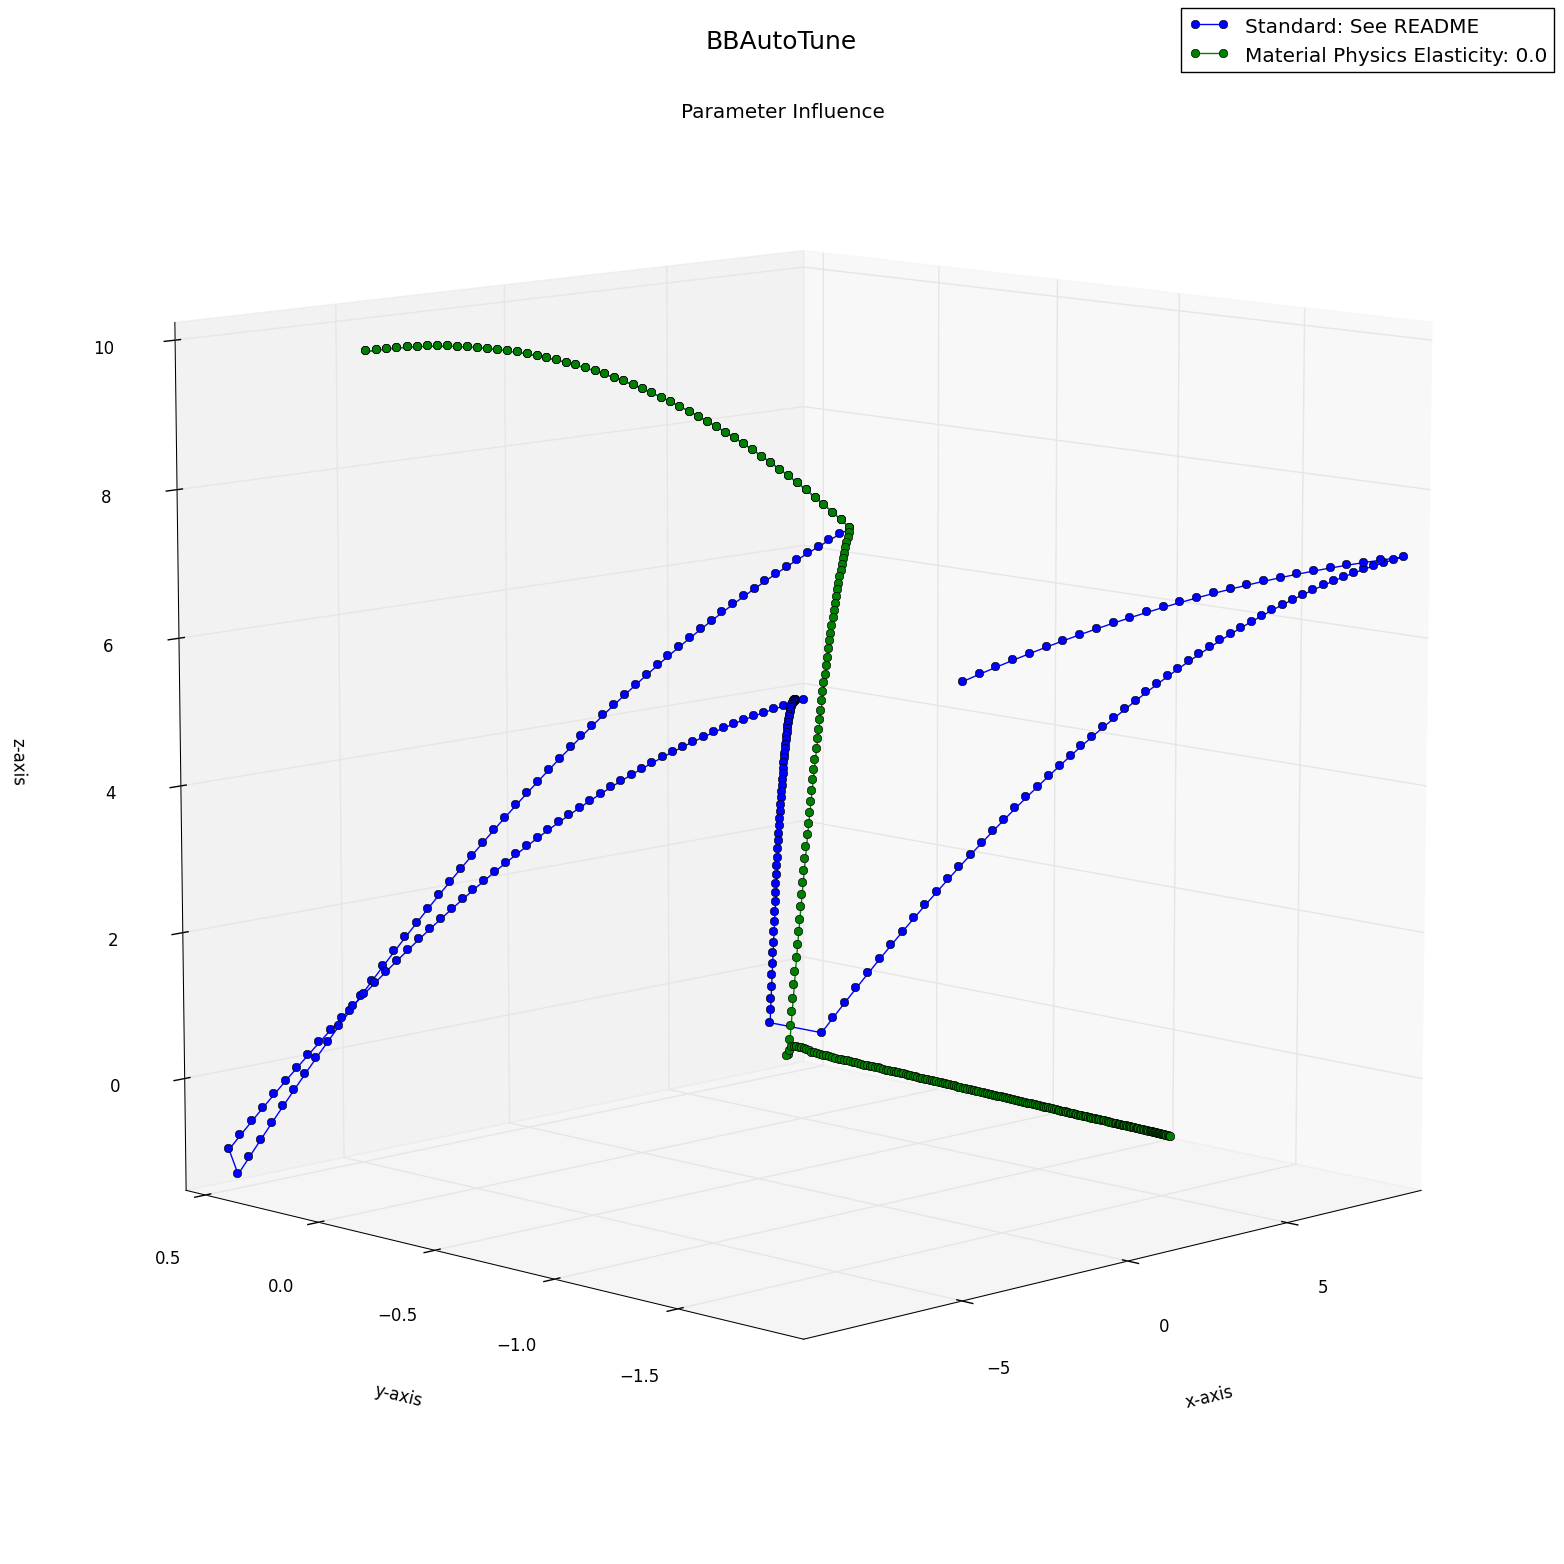
\includegraphics[scale=0.35]{../Figures/Chapter4/material_physics_ball_plot.png}
\rule{35em}{0.5pt}
\caption[Physics Engine Racquetball Path Dissimilarity]{The dissimilarity of the ball paths between the tweaked, material-physics elasticity parameter and the standard (where no parameters were tweaked).}
\label{fig:matphysplot}
\end{figure}

\begin{figure}[htbp]
\centering
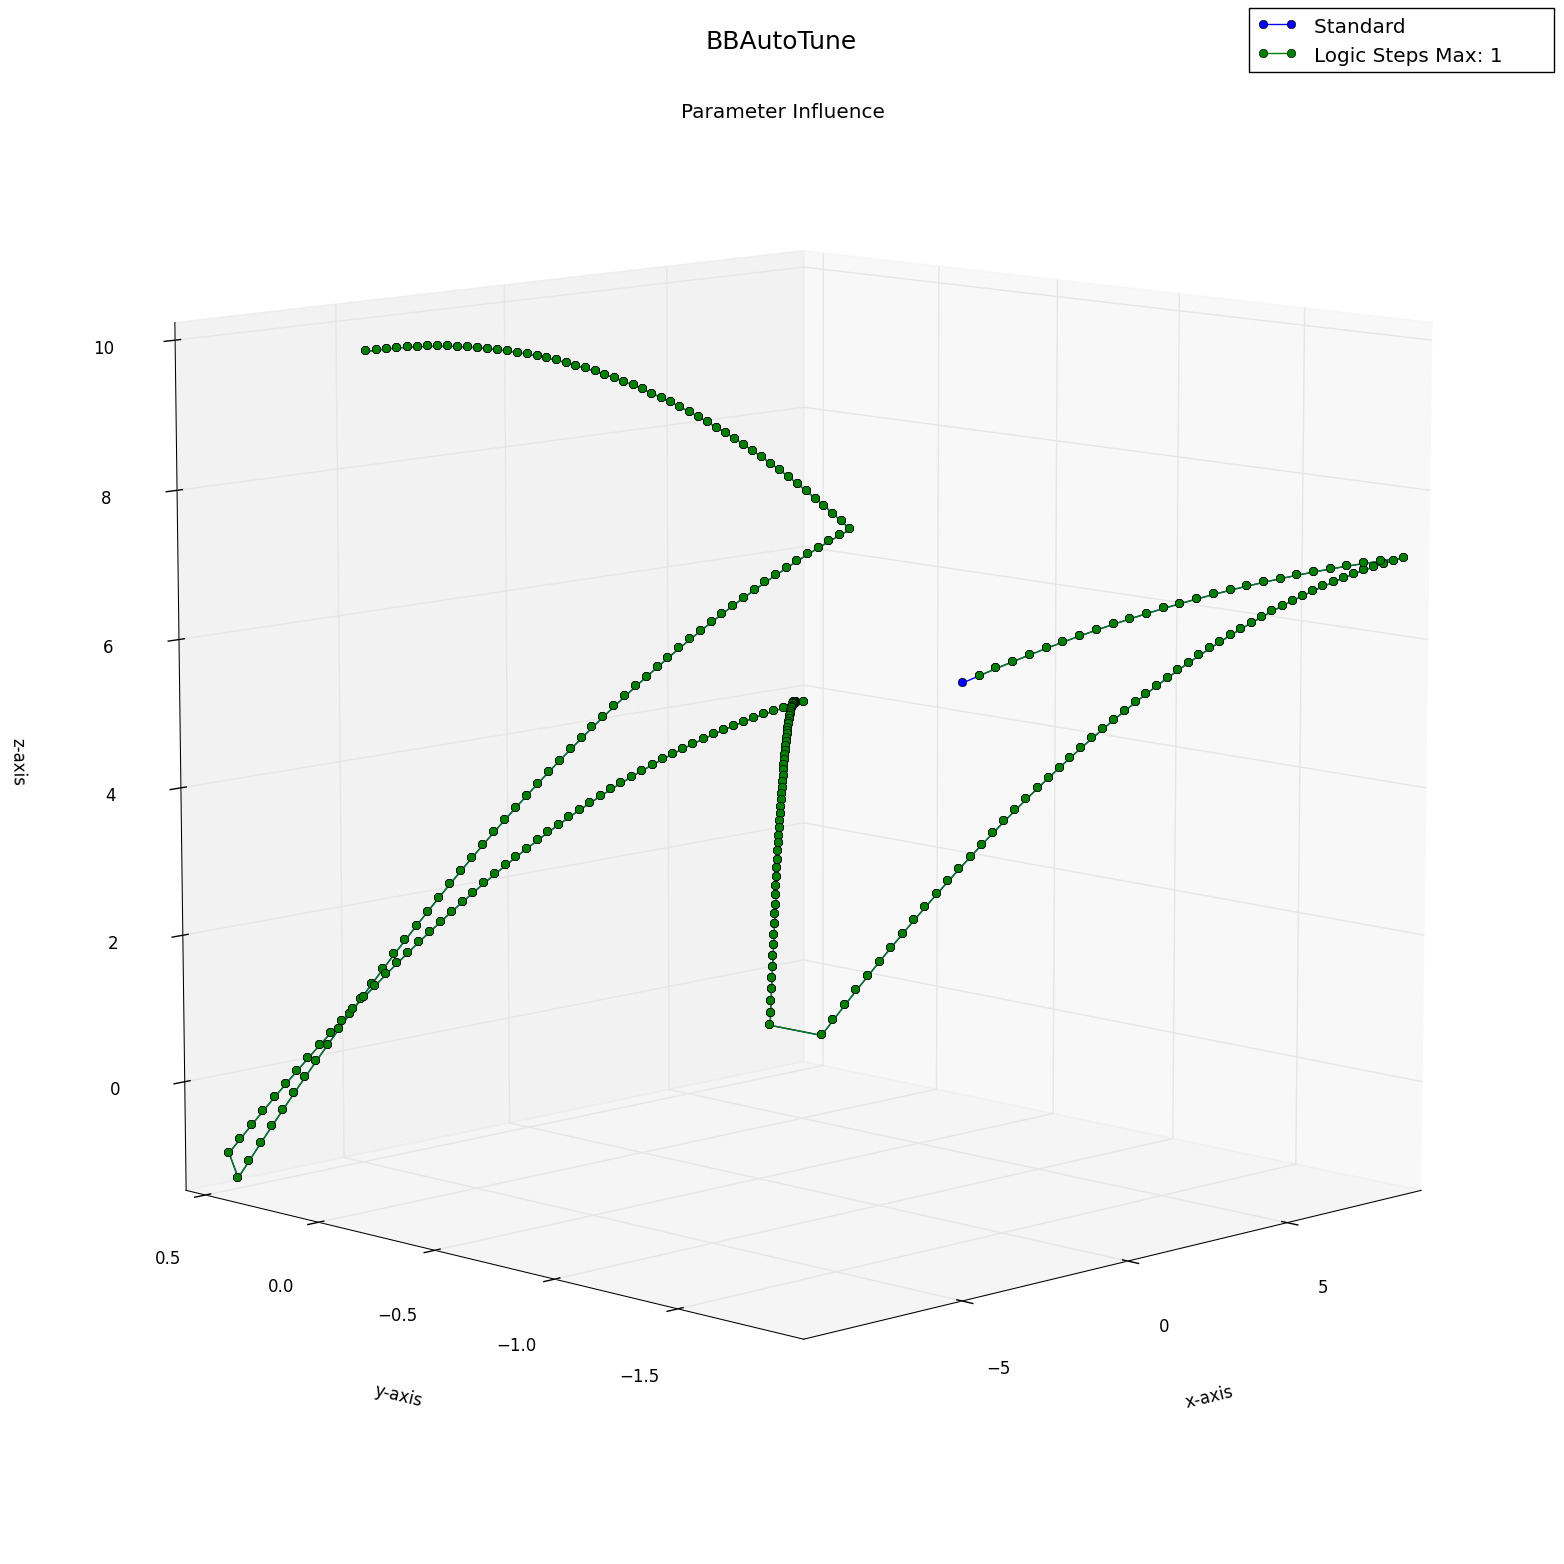
\includegraphics[scale=0.35]{../Figures/Chapter4/logic_steps_ball_plot.png}
\rule{35em}{0.5pt}
\caption[Physics Engine Racquetball Path Similarity]{The similarity of the ball paths between the tweaked, logic-steps maximum parameter and the standard (where no parameters were tweaked).}
\label{fig:logicstepsplot}
\end{figure}

\begin{figure}[htbp]
\begin{center}
\begin{varwidth}{\textwidth}
{\tt
BEGIN \\
\tab $P = \langle p_1, p_2,...,p_n\rangle$ \\
\tab $Q = \langle q_1, q_2,...,q_m\rangle$ \\
\tab $max = 0.0$ \\
\tab For all $p_i\in P$ and $q_j \in Q$ do \\
\tab \tab $d = ||p_i-q_j||$ \\
\tab \tab If $max$ $<$ $d$ then \\
\tab \tab \tab $max=d$ \\
\tab \tab End if \\
\tab End for \\
\tab Return $max$ \\
END \\
}
\end{varwidth}
\end{center}
\centering
% \begin{equation*}
% \begin{align}
% Algorithm: & \\
% & P = \langle p_1, p_2,...,p_n\rangle \\
% & Q = \langle q_1, q_2,...,q_m\rangle \\
% & max = 0.0 \\
% & For \ all \ p_i\in P \ and \ q_j \in Q \ do: \\
% & \quad d = ||p_i-q_j|| \\
% & \quad If \ max < d \ then: \\
% & \qquad max \leftarrow d \\
% & return \ max \\
% \end{align}
% \end{equation*}
\rule{35em}{0.5pt}
\caption[Lettier Distance Algorithm]{The Lettier distance algorithm.}
\label{lettierdistance}
\end{figure}

Twenty parameters out of the initial 44 showed no significant influence over the 3D physics simulation in Blender. Thus, the resulting 24 parameters which did have a significant influence were targeted for tuning by the genetic algorithm. See Table \ref{tab:distances}.

\begin{table}[htbp]
\centering
\footnotesize
\def\arraystretch{1.1}
\begin{tabular}{ | l || l | l | l | }
\hline
\rowcolor{gray}
Tweaked Parameter: Value & Lettier Distance & Discrete Fr{\'e}chet Distance & Hausdorff Distance \\ \hline
Gravity: $1.0\frac{m}{s^2}$ & 12.7741189989 & 20.948159542 & 9.86343687719 \\ \hline
\rowcolor{cyan}
Physics Steps Max: 1 & 0.329232644023 & 0.329232644023 & 0.329232644023 \\ \hline
Physics Sub-steps: 50 & 19.3073641073 & 17.0708640308 & 11.3180046289 \\ \hline
Physics FPS: 1 & 218.037284056 & 211.287842927 & 205.848670021 \\ \hline
\rowcolor{cyan}
Logic Steps Max: 1 & 0.329232644023 & 0.329232644023 & 0.329232644023 \\ \hline
\rowcolor{cyan}
Physics Deactivation Linear Threshold: 10000.0 & 0.329232644023 & 0.329232644023 & 0.329232644023 \\ \hline
\rowcolor{cyan}
Physics Deactivation Angular Threshold: 10000.0 & 0.329232644023 & 0.329232644023 & 0.329232644023 \\ \hline
\rowcolor{cyan}
Physics Deactivation Time: 0.0 & 0.329232644023 & 0.329232644023 & 0.329232644023 \\ \hline
\rowcolor{cyan}
Occlusion Culling: False & 0.329232644023 & 0.329232644023 & 0.329232644023 \\ \hline
\rowcolor{cyan}
Occlusion Culling Resolution: 1024 & 0.329232644023  & 0.329232644023  & 0.329232644023 \\ \hline
Material Physics: False & 18.0830473811 & 18.0830473811  & 18.0830473811 \\ \hline
Material Physics Friction: 100.00 & 4.93924881608  & 4.94095279557  & 3.8109066203 \\ \hline
Material Physics Elasticity: 0.0 & 17.3874844829  & 17.0233755244  & 11.3180046289 \\ \hline
\rowcolor{cyan}
Force Field Force: 1.00 & 0.329232644023  & 0.329232644023  & 0.329232644023 \\ \hline
\rowcolor{cyan}
Force Field Damping: 1.00 & 0.329232644023  & 0.329232644023  & 0.329232644023 \\ \hline
\rowcolor{cyan}
Force Field Distance: 20.00 & 0.329232644023  & 0.329232644023  & 0.329232644023 \\ \hline
\rowcolor{cyan}
Force Field Align to Normal: True & 0.329232644023  & 0.329232644023  & 0.329232644023 \\ \hline
Physics Type: Dynamic & 3.55513601614  & 18.1217630973  & 3.275450812 \\ \hline
\rowcolor{cyan}
Use Actor: False & 0.329232644023  & 0.329232644023  & 0.329232644023 \\ \hline
Use Ghost: True & 138.489494312  & 138.489494312  & 132.02387242 \\ \hline
\rowcolor{cyan}
Use Material Force Field: True & 0.329232644023  & 0.329232644023  & 0.329232644023 \\ \hline
\rowcolor{cyan}
Rotate From Normal: True & 0.329232644023  & 0.329232644023  & 0.329232644023 \\ \hline
\rowcolor{cyan}
No Sleeping: True & 0.329232644023  & 0.329232644023  & 0.329232644023 \\ \hline
Mass: 10000.0 & 3.57800913743  & 3.30042073543  & 3.21534852885 \\ \hline
\rowcolor{cyan}
Radius: 1cm & 0.329232644023  & 0.329232644023  & 0.329232644023 \\ \hline
Form Factor: 0.0 & 3.55513601614  & 18.1217630973  & 3.275450812 \\ \hline
\rowcolor{cyan}
Velocity Minimum: 1.0 & 0.329232644023  & 0.329232644023  & 0.329232644023 \\ \hline
\rowcolor{cyan}
Anisotropic Friction: True & 0.329232644023  & 0.329232644023  & 0.329232644023 \\ \hline
Velocity Maximum: 1.0 & 17.1034960114  & 17.130808295  & 16.8922077042 \\ \hline
Damping Translation: 1.0 & 17.9729741832 & 17.9729741832 & 17.9729741832 \\ \hline
Damping Rotation: 1.0 & 8.09457671285 & 5.47840838373 & 5.18331655137 \\ \hline
Collision Bounds: False & 8.81773036062 & 17.4044978663 & 2.80531111777 \\ \hline
Collision Bounds Margin: 0m & 18.740072391  & 9.79629223411  & 3.78119352088 \\ \hline
Collision Bounds: False & 4.28865271192  & 4.23797419961  & 3.72440427516 \\ \hline
Launch Dynamic Object Settings Force X: 30.0 & 5.21169989737  & 5.21169989737  & 3.78308993247 \\ \hline
Launch Dynamic Object Settings Torque X: 30.0 & 8.82943537929  & 8.70403741077  & 6.58255281735 \\ \hline
Launch Dynamic Object Settings AngV X: 30.0 & 2.93219084728  & 2.63246279507  & 1.82341393368 \\ \hline
Launch Dynamic Object Settings LinV X: 0.0 & 19.1625050915  & 19.1625050915  & 17.0670582483 \\ \hline
\rowcolor{cyan}
Launch Damping Frames: -32768 & 0.329232644023 & 0.329232644023  & 0.329232644023 \\ \hline
Collision Dynamic Object Settings Force X: 30.0 & 5.32618850819  & 18.9696056987  & 3.80913153981 \\ \hline
Collision Dynamic Object Settings Torque X: 30.0 & 1.67496526126  & 1.52842619107  & 1.52842619107 \\ \hline
Collision Dynamic Object Settings LinV X: 0.0 & 19.2801183238  & 19.1535557726  & 3.3918725084 \\ \hline
Collision Dynamic Object Settings AngV X: 30.0 & 4.69097055763 & 18.7403224372 & 3.80913153981 \\ \hline
\rowcolor{cyan}
Damping Frames: -32768 & 0.329232644023 & 0.329232644023 & 0.329232644023 \\ \hline
\end{tabular}
\caption[Physics Engine Parameter Influences]{The distances between each tweaked-parameter ball path and the standard ball path for each of the three quantifiable measurement methods employed. The highlighted tweaked parameters were determined not to be influential.}
\label{tab:distances}
\end{table}

\newpage

\subsection[Experiment Two]{Experiment two: tournament selection with self-adaptation.}
\label{subsec:bbautotune_exp_two}

The minimum values reached for the highest, average, and lowest fitness were 0.9306191001, 1.024632475, and 0.9315692954 respectively. The minimum and maximum probability for both crossover and mutation obtained over the course of 500 generations was 0.001 and 0.999. Interestingly, as the highest, average, and lowest fitness began to converge, the crossover and mutation probability flipped, causing the population to be entirely mutated (with the exception of the elites) which resulted in essentially a randomly generated population and thereby destroying the high fitness solutions previously found. Notice that after the probabilities flipped, the average and lowest fitness diverged. This converging and then diverging occurred twice during the 500 generation run. Up to generation 376, the highest fitness steadily declined and then afterward remained fairly stable. See Figure \ref{fig:exp2_halcm}. Table \ref{tab:exp2_best_worst_params} lists the best and worst physics parameters found by the GA, corresponding to the best and worst fitness observed during the 500 generation run.

\begin{figure}[htbp]
\centering
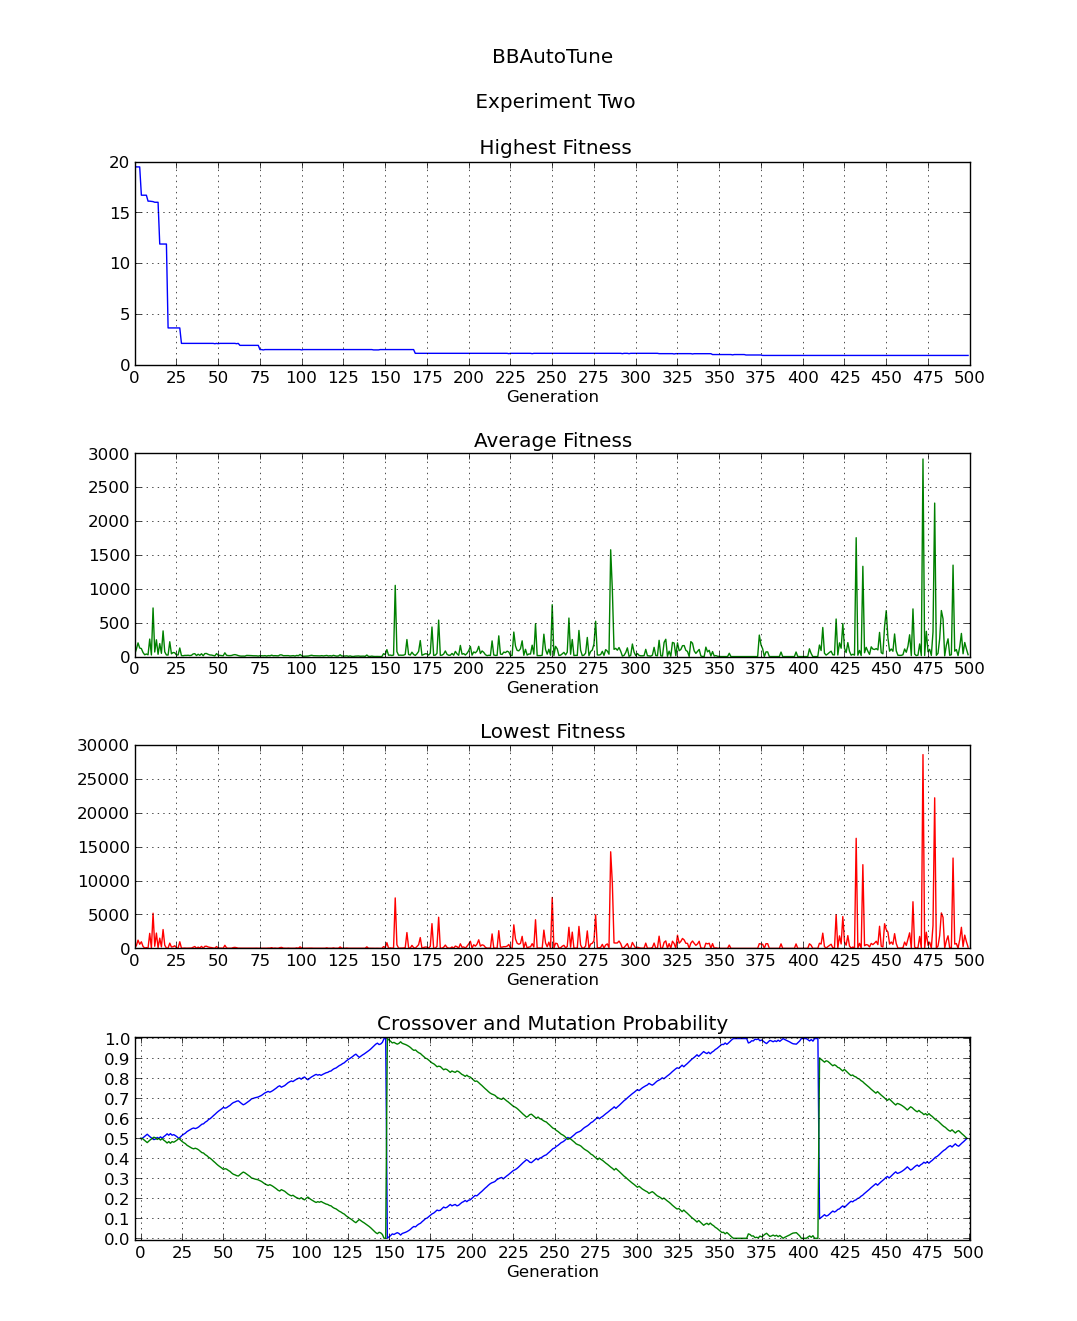
\includegraphics[width=5in]{../Figures/Chapter4/exp2_halcm.png}
\rule{35em}{0.5pt}
\caption[Experiment Two GA Metrics]{The highest, average, and lowest fitness in addition to the crossover and mutation probability over the course of 500 generations. For the bottom plot, the crossover probability is shown in blue while the mutation probability is shown in green.}
\label{fig:exp2_halcm}
\end{figure}

\begin{table}[htbp]
\centering
\footnotesize
\bgroup
\def\arraystretch{1.1}
\begin{tabular}{ | >{\centering\arraybackslash}m{3cm} | >{\centering\arraybackslash}m{3cm} | >{\centering\arraybackslash}m{3cm} | }
%\hline
%\rowcolor{gray}
\cline{2-3}
\multicolumn{1}{c|}{}                 & \cellcolor{gray} Best         & \cellcolor{gray} Worst        \\ \hline
\cellcolor{gray} Gravity              & 2.89862416489$\frac{m}{s^2}$  & 10.1989482496$\frac{m}{s^2}$  \\ \hline
\cellcolor{gray} Sub-steps            & 5                             & 5                             \\ \hline
\cellcolor{gray} FPS                  & 30                            & 30                            \\ \hline
\cellcolor{gray} Material Friction    & 59.5011814113                 & 77.8151135094                 \\ \hline
\cellcolor{gray} Material Elasticity  & 0.0742521056997               & 0.279061300281                \\ \hline
\cellcolor{gray} Mass                 & 4.33392950881                 & 1.76678194417                 \\ \hline
\cellcolor{gray} Velocity Maximum        & 900.11395466                  & 647.638168514                 \\ \hline
\cellcolor{gray} Damping Translation  & 1.0                           & 0.0                           \\ \hline
\cellcolor{gray} Damping Rotation     & 0.691143247902                & 0.648240602049                \\ \hline
\cellcolor{gray} Collision Bounds Type & SPHERE                        & SPHERE                        \\ \hline
\cellcolor{gray} Torque               & 82.7271515601                 & 100.0                         \\ \hline \hline
\cellcolor{gray} Fitness              & 0.930619100106                & 28584.2244771                 \\ \hline
\end{tabular}
\egroup
\caption[Experiment Two Best and Worst Physics Parameters Found]{The best and worst physics parameters found by the GA corresponding to the best and worst fitness observed during the 500 generation run for experiment two.}
\label{tab:exp2_best_worst_params}
\end{table}

% gravity,2.89862416489
% sub_steps,5
% fps,30
% material_friction,59.5011814113
% material_elasticity,0.0742521056997
% mass,4.33392950881
% velocity_max,900.11395466
% damping,1.0
% rotation_damping,0.691143247902
% collision_bounds_type,SPHERE
% torque_z,82.7271515601
% fitness,0.930619100106

% gravity,10.1989482496
% sub_steps,5
% fps,30
% material_friction,77.8151135094
% material_elasticity,0.279061300281
% mass,1.76678194417
% velocity_max,647.638168514
% damping,0.0
% rotation_damping,0.648240602049
% collision_bounds_type,SPHERE
% torque_z,100.0
% fitness,28584.2244771

\newpage

\subsection[Experiment Three]{Experiment three: tournament selection without self-adaptation.}

The minimum values reached for the highest, average, and lowest fitness were 1.0827696957, 2.892412821, and 7.7702053307 respectively. Up until generation 146, the highest fitness steadily declined and then afterwards remained fairly stable. See Figure \ref{fig:exp3_halcm}. In contrast to experiment two, it would seem that the self-adaptation side effect of periodically randomizing the population helped experiment two obtain a better fitness than experiment three. Table \ref{tab:exp3_best_worst_params} lists the best and worst physics parameters found by the GA, corresponding to the best and worst fitness observed during the 500 generation run.

\begin{figure}[htbp]
\centering
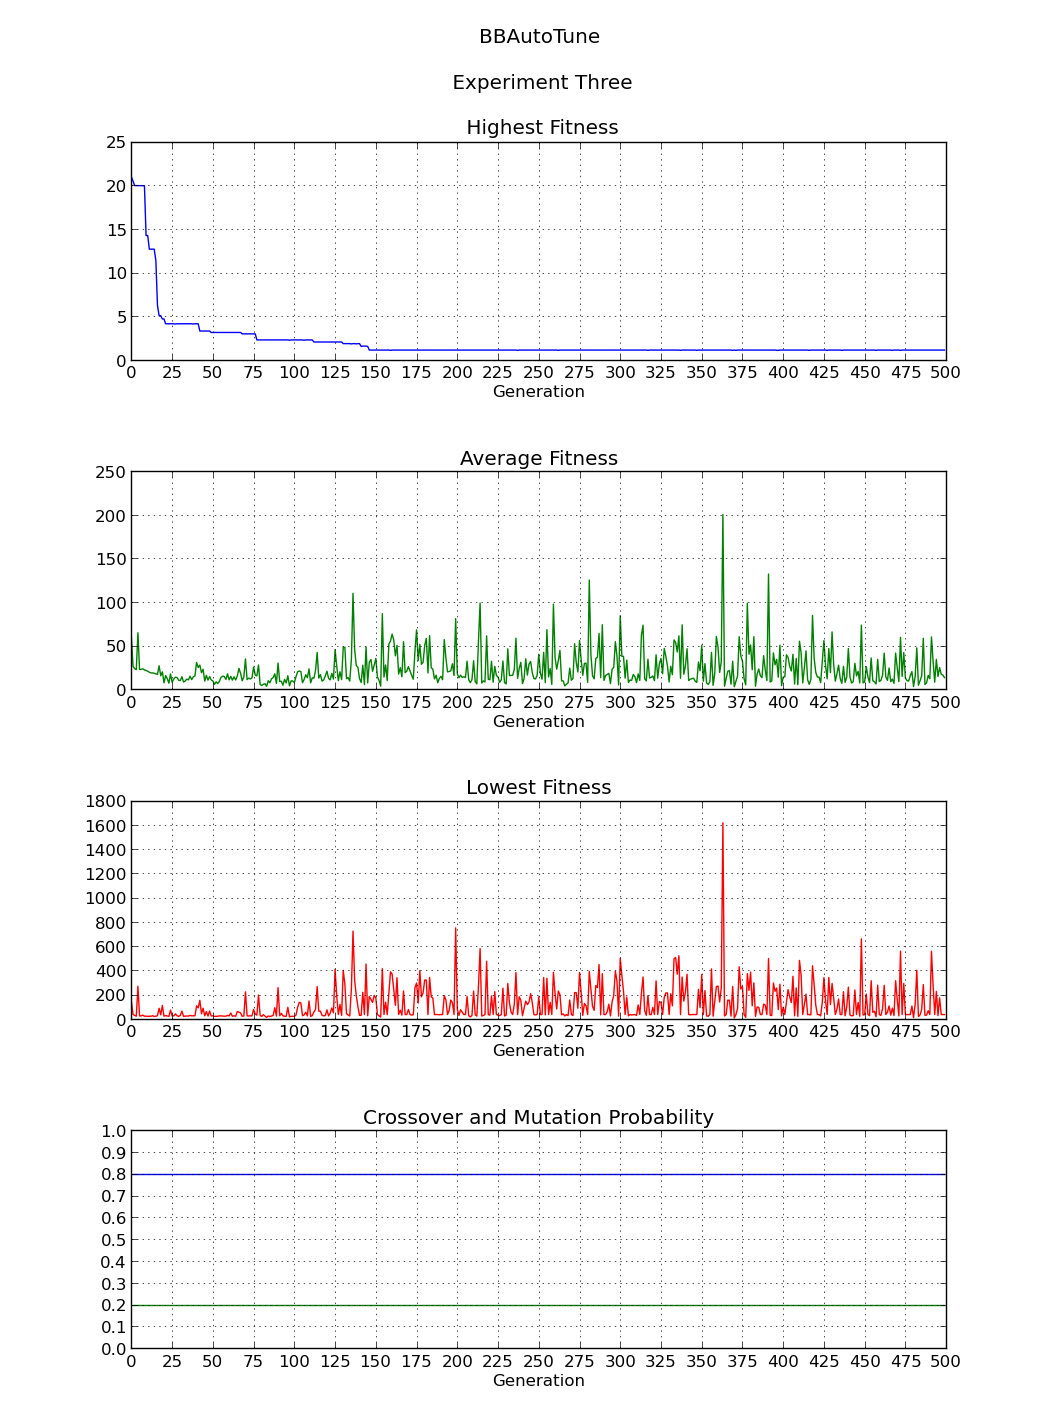
\includegraphics[width=5in]{../Figures/Chapter4/exp3_halcm.png}
\rule{35em}{0.5pt}
\caption[Experiment Three GA Metrics]{The highest, average, and lowest fitness in addition to the crossover and mutation probability over the course of 500 generations. For the bottom plot, the crossover probability is shown in blue while the mutation probability is shown in green.}
\label{fig:exp3_halcm}
\end{figure}

\begin{table}[htbp]
\centering
\footnotesize
\bgroup
\def\arraystretch{1.1}
\begin{tabular}{ | >{\centering\arraybackslash}m{3cm} | >{\centering\arraybackslash}m{3cm} | >{\centering\arraybackslash}m{3cm} | }
%\hline
%\rowcolor{gray}
\cline{2-3}
\multicolumn{1}{c|}{}                 & \cellcolor{gray} Best             & \cellcolor{gray} Worst             \\ \hline
\cellcolor{gray} Gravity              & 14.09509165745291$\frac{m}{s^2}$  & 0.8362602682788933$\frac{m}{s^2}$  \\ \hline
\cellcolor{gray} Sub-steps            & 1                                 & 1                                  \\ \hline
\cellcolor{gray} FPS                  & 30                                & 30                                 \\ \hline
\cellcolor{gray} Material Friction    & 79.87292012678728                 & 100.0                              \\ \hline
\cellcolor{gray} Material Elasticity  & 0.7331947746415657                & 0.6643893038716038                 \\ \hline
\cellcolor{gray} Mass                 & 15.0                              & 12.761484385447746                 \\ \hline
\cellcolor{gray} Velocity Maximum     & 0.0                               & 250.88084935511978                 \\ \hline
\cellcolor{gray} Damping Translation  & 1.0                               & 0.33429608723965537                \\ \hline
\cellcolor{gray} Damping Rotation     & 0.14340109658364997               & 0.0                                \\ \hline
\cellcolor{gray} Collision Bounds Type & TRIANGLE\_MESH                    & SPHERE                             \\ \hline
\cellcolor{gray} Torque               & 47.85677413931377                 & 63.68300968863001                  \\ \hline \hline
\cellcolor{gray} Fitness              & 1.0827696957                      & 1617.02428027                      \\ \hline
\end{tabular}
\egroup
\caption[Experiment Three Best and Worst Physics Parameters Found]{The best and worst physics parameters found by the GA corresponding to the best and worst fitness observed during the 500 generation run for experiment three.}
\label{tab:exp3_best_worst_params}
\end{table}

% gravity,14.09509165745291
% sub_steps,1
% fps,30
% material_friction,79.87292012678728
% material_elasticity,0.7331947746415657
% mass,15.0
% velocity_max,0.0
% damping,1.0
% rotation_damping,0.14340109658364997
% collision_bounds_type,TRIANGLE_MESH
% torque_z,47.85677413931377
% fitness,1.0827696957

% gravity,0.8362602682788933
% sub_steps,1
% fps,30
% material_friction,100.0
% material_elasticity,0.6643893038716038
% mass,12.761484385447746
% velocity_max,250.88084935511978
% damping,0.33429608723965537
% rotation_damping,0.0
% collision_bounds_type,SPHERE
% torque_z,63.68300968863001
% fitness,1617.02428027

\newpage

\subsection[Experiment Four]{Experiment four: rank fitness selection with self-adaptation.}

The minimum values reached for the highest, average, and lowest fitness were 1.1309704845, 2.7714017205, and 2.5217479907 respectively. The minimum and maximum probabilities observed for crossover, during the 500 generation run, were 0.253 and 0.999 respectively. For mutation, the minimum and maximum probabilities observed were 0.001 and 0.747 respectively. From generation zero to 79, the highest fitness steadily declined and then fell more gradually afterwards for rest of the duration. The same periodic converging and then diverging seen in experiment two was observed again in experiment four. See Figure \ref{fig:exp4_halcm}. Table \ref{tab:exp4_best_worst_params} lists the best and worst physics parameters found by the GA, corresponding to the best and worst fitness observed during the 500 generation run.

\begin{figure}[htbp]
\centering
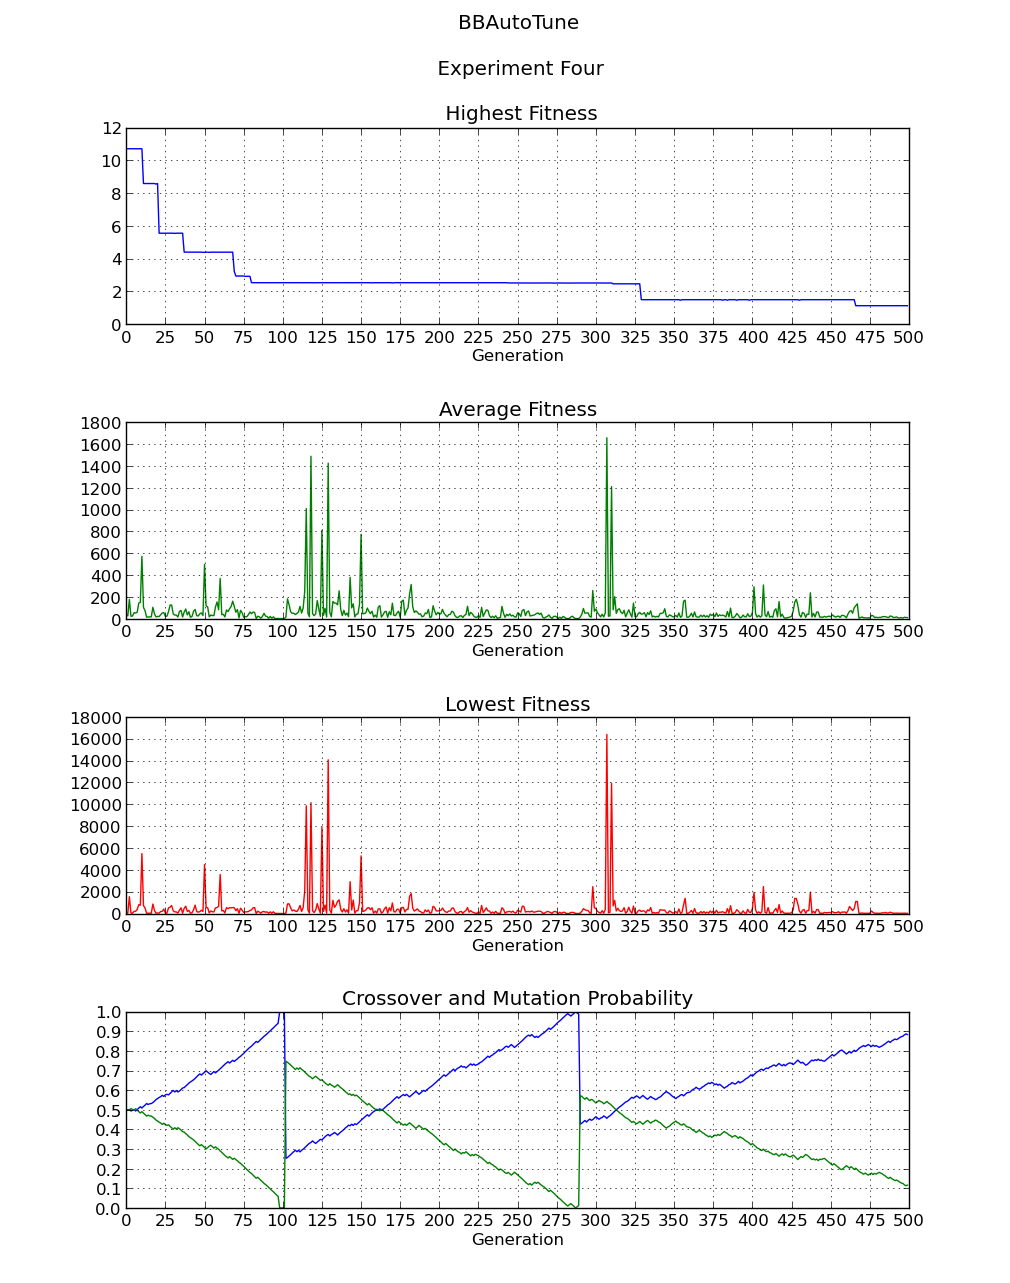
\includegraphics[width=5in]{../Figures/Chapter4/exp4_halcm.png}
\rule{35em}{0.5pt}
\caption[Experiment Four GA Metrics]{The highest, average, and lowest fitness in addition to the crossover and mutation probability over the course of 500 generations. For the bottom plot, the crossover probability is shown in blue while the mutation probability is shown in green.}
\label{fig:exp4_halcm}
\end{figure}

\begin{table}[htbp]
\centering
\footnotesize
\bgroup
\def\arraystretch{1.1}
\begin{tabular}{ | >{\centering\arraybackslash}m{3cm} | >{\centering\arraybackslash}m{3cm} | >{\centering\arraybackslash}m{3cm} | }
%\hline
%\rowcolor{gray}
\cline{2-3}
\multicolumn{1}{c|}{}                 & \cellcolor{gray} Best         & \cellcolor{gray} Worst  \\ \hline
\cellcolor{gray} Gravity              & 13.8256917774$\frac{m}{s^2}$  & 15.0$\frac{m}{s^2}$     \\ \hline
\cellcolor{gray} Sub-steps            & 2                             & 5                       \\ \hline
\cellcolor{gray} FPS                  & 30                            & 30                      \\ \hline
\cellcolor{gray} Material Friction    & 61.2749944576                 & 0.0                     \\ \hline
\cellcolor{gray} Material Elasticity  & 0.171754015461                & 0.649745829218          \\ \hline
\cellcolor{gray} Mass                 & 15.0                          & 0.158414320671          \\ \hline
\cellcolor{gray} Velocity Maximum        & 1000.0                        & 1000.0                  \\ \hline
\cellcolor{gray} Damping Translation  & 0.0                           & 0.387362543282          \\ \hline
\cellcolor{gray} Damping Rotation     & 0.984539067046                & 0.687852083808          \\ \hline
\cellcolor{gray} Collision Bounds Type & SPHERE                        & CONVEX\_HULL            \\ \hline
\cellcolor{gray} Torque               & 6.70058480184                 & 75.8262976514           \\ \hline \hline
\cellcolor{gray} Fitness              & 1.1309704845                  & 16396.2145412           \\ \hline
\end{tabular}
\egroup
\caption[Experiment Four Best and Worst Physics Parameters Found]{The best and worst physics parameters found by the GA corresponding to the best and worst fitness observed during the 500 generation run for experiment four.}
\label{tab:exp4_best_worst_params}
\end{table}

% gravity,13.8256917774
% sub_steps,2
% fps,30
% material_friction,61.2749944576
% material_elasticity,0.171754015461
% mass,15.0
% velocity_max,1000.0
% damping,0.0
% rotation_damping,0.984539067046
% collision_bounds_type,SPHERE
% torque_z,6.70058480184
% fitness,1.13097048447

% gravity,15.0
% sub_steps,5
% fps,30
% material_friction,0.0
% material_elasticity,0.649745829218
% mass,0.158414320671
% velocity_max,1000.0
% damping,0.387362543282
% rotation_damping,0.687852083808
% collision_bounds_type,CONVEX_HULL
% torque_z,75.8262976514
% fitness,16396.2145412

\newpage

\subsection[Experiment Five]{Experiment five: rank fitness selection without self-adaptation.}

The minimum values reached for the highest, average, and lowest fitness were 1.0638026764, 3.4974350451, and 11.6425679783 respectively. Throughout the 500 generation run, the highest fitness continued to decline reaching its lowest value at generation 469. See Figure \ref{fig:exp5_halcm}. Table \ref{tab:exp5_best_worst_params} lists the best and worst physics parameters found by the GA corresponding to the best and worst fitness observed during the 500 generation run.

\begin{figure}[htbp]
\centering
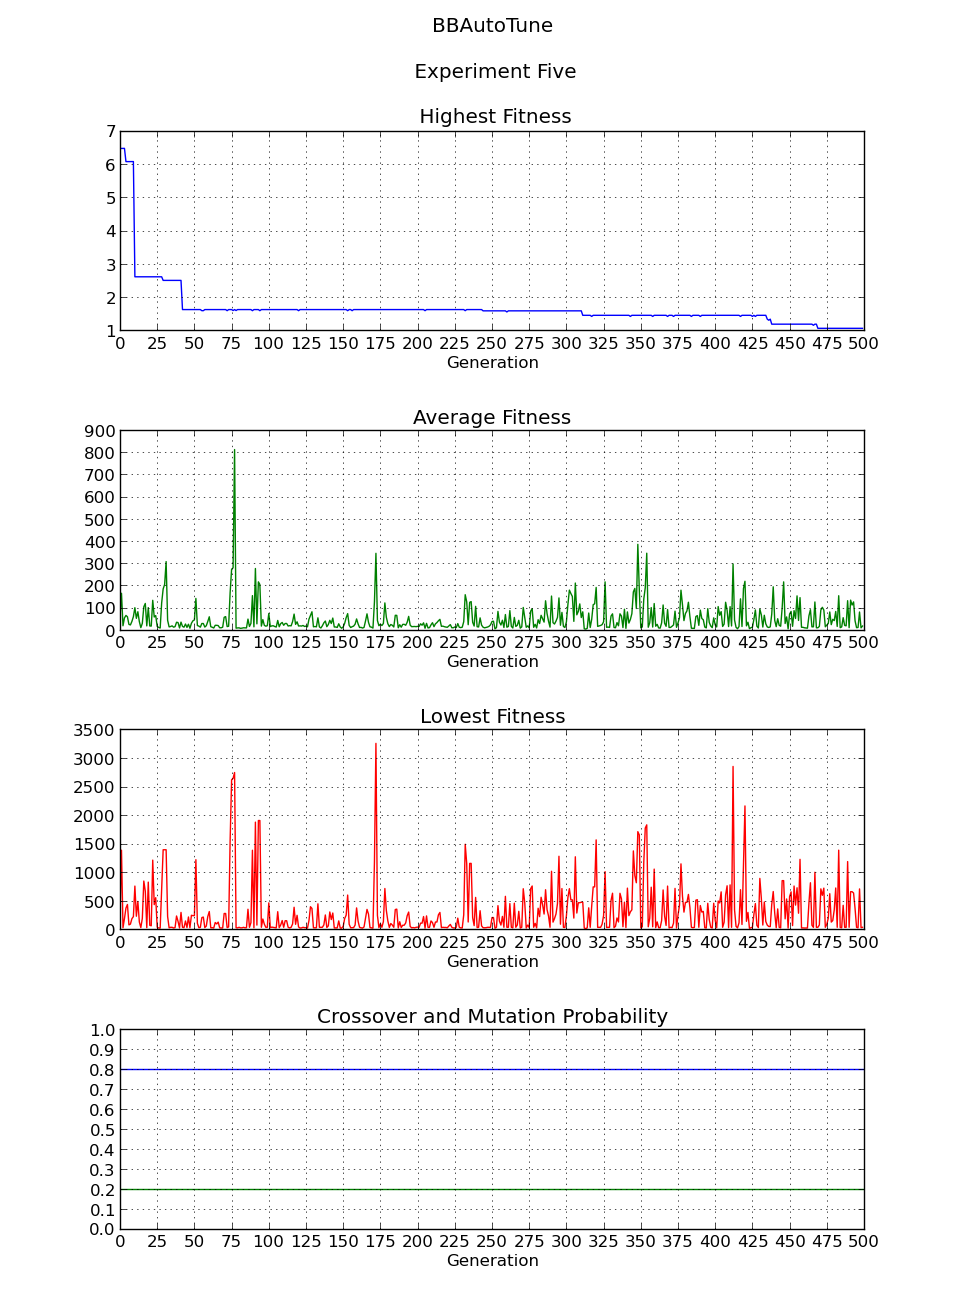
\includegraphics[width=5in]{../Figures/Chapter4/exp5_halcm.png}
\rule{35em}{0.5pt}
\caption[Experiment Five GA Metrics]{The highest, average, and lowest fitness in addition to the crossover and mutation probability over the course of 500 generations. For the bottom plot, the crossover probability is shown in blue while the mutation probability is shown in green.}
\label{fig:exp5_halcm}
\end{figure}

\begin{table}[htbp]
\centering
\footnotesize
\bgroup
\def\arraystretch{1.1}
\begin{tabular}{ | >{\centering\arraybackslash}m{3cm} | >{\centering\arraybackslash}m{3cm} | >{\centering\arraybackslash}m{3cm} | }
%\hline
%\rowcolor{gray}
\cline{2-3}
\multicolumn{1}{c|}{}                 & \cellcolor{gray} Best         & \cellcolor{gray} Worst                \\ \hline
\cellcolor{gray} Gravity              & 0.0$\frac{m}{s^2}$            & 12.803362098213498$\frac{m}{s^2}$     \\ \hline
\cellcolor{gray} Sub-steps            & 3                             & 2                                     \\ \hline
\cellcolor{gray} FPS                  & 30                            & 30                                    \\ \hline
\cellcolor{gray} Material Friction    & 60.71902294177607             & 15.76102238218593                     \\ \hline
\cellcolor{gray} Material Elasticity  & 0.5378313234044673            & 0.602617926833965                     \\ \hline
\cellcolor{gray} Mass                 & 4.175314301157847             & 0.2111916960575379                    \\ \hline
\cellcolor{gray} Velocity Maximum        & 660.0787581868401             & 787.7673658611162                     \\ \hline
\cellcolor{gray} Damping Translation  & 1.0                           & 0.6703819812309364                    \\ \hline
\cellcolor{gray} Damping Rotation     & 0.4031179325185546            & 0.10076651150002103                   \\ \hline
\cellcolor{gray} Collision Bounds Type & SPHERE                        & SPHERE                                \\ \hline
\cellcolor{gray} Torque               & 46.465508081185064            & 49.46737364841879                     \\ \hline \hline
\cellcolor{gray} Fitness              & 1.0638026764                  & 3257.00654843                         \\ \hline
\end{tabular}
\egroup
\caption[Experiment Five Best and Worst Physics Parameters Found]{The best and worst physics parameters found by the GA corresponding to the best and worst fitness observed during the 500 generation run for experiment five.}
\label{tab:exp5_best_worst_params}
\end{table}

% gravity,0.0
% sub_steps,3
% fps,30
% material_friction,60.71902294177607
% material_elasticity,0.5378313234044673
% mass,4.175314301157847
% velocity_max,660.0787581868401
% damping,1.0
% rotation_damping,0.4031179325185546
% collision_bounds_type,SPHERE
% torque_z,46.465508081185064
% fitness,1.06380267644

% gravity,12.803362098213498
% sub_steps,2
% fps,30
% material_friction,15.76102238218593
% material_elasticity,0.602617926833965
% mass,0.2111916960575379
% velocity_max,787.7673658611162
% damping,0.6703819812309364
% rotation_damping,0.10076651150002103
% collision_bounds_type,SPHERE
% torque_z,49.46737364841879
% fitness,3257.00654843

\newpage

\section{Simulated versus Real Motion}
\label{sec:sim_vs_real_mot}

The top phenotype for experiment two had the largest robust distance from the real robot robust mean, but suffered the least amount of penalty for not stopping at one second. The top phenotypes for experiments three through five had similar robust distances and stopping times over one second. See Table \ref{tab:comp_top_phenotypes}, Figure \ref{fig:simu_vs_real_line}, and Figure \ref{fig:simu_vs_real_3d}. 

\begin{table}[htbp]
\centering
\footnotesize
\bgroup
\def\arraystretch{1.1}
\begin{tabular}{ | >{\centering\arraybackslash}m{2cm} | >{\centering\arraybackslash}m{2cm} | >{\centering\arraybackslash}m{2cm} | >{\centering\arraybackslash}m{2cm} | >{\centering\arraybackslash}m{2cm} | >{\centering\arraybackslash}m{2cm} | }
%\hline
%\rowcolor{gray}
\cline{2-5}
\multicolumn{1}{c|}{} & \multicolumn{4}{c}{ \cellcolor{gray} Final States of Highest Performing Phenotypes} & \multicolumn{1}{c}{} \\
\cline{2-5}
\multicolumn{1}{c|}{}                                & \cellcolor{gray} Exp. Two & \cellcolor{gray} Exp. Three & \cellcolor{gray} Exp. Four & \cellcolor{gray} Exp. Five & \cellcolor{gray} Real Robot Robust Mean \\ \hline
\cellcolor{gray} X-position                       & 23.12349975cm    &  23.95108938cm  & 23.49144816cm   & 24.05546605cm  &  23.9934044cm  \\  \hline
\cellcolor{gray} Y-position                       &  0.00953689cm    &  -0.34897618cm  & -0.00286334cm   &  0.01641194cm  &   0.0351240cm  \\  \hline
\cellcolor{gray} Heading (Z-orientation)          &  0.00203373rad   &  -0.00318596rad & -0.00428754rad  &  0.00118415rad &  -0.0189964rad \\  \hline
\multicolumn{6}{c}{} \\
\cline{1-5}
\cellcolor{gray} Elapsed Time Until Coming to a Stop &  1.0333563sec    &   1.5333535sec  &  1.5333476sec   &  1.5333496sec  &  \multicolumn{1}{c}{} \\
\cline{1-5}
\multicolumn{6}{c}{} \\
\cline{1-5}
\cellcolor{gray} Resulting Genome Fitness & 0.930619100106 & 1.0827696957 & 1.1309704845 & 1.0638026764 &  \multicolumn{1}{c}{} \\
\cline{1-5}
\end{tabular}
\egroup
\caption[Comparison of the Top Phenotypes' Final States to the Real Robot Motion]{The comparison between the top phenotypes' final states (per experiment) and the robust mean of the real robot forward motion. The elapsed times indicate how long each top phenotype took before reaching its final at-rest state. The resulting genome fitnesses are included for reference.}
\label{tab:comp_top_phenotypes}
\end{table}

\begin{figure}[htbp]
\centering
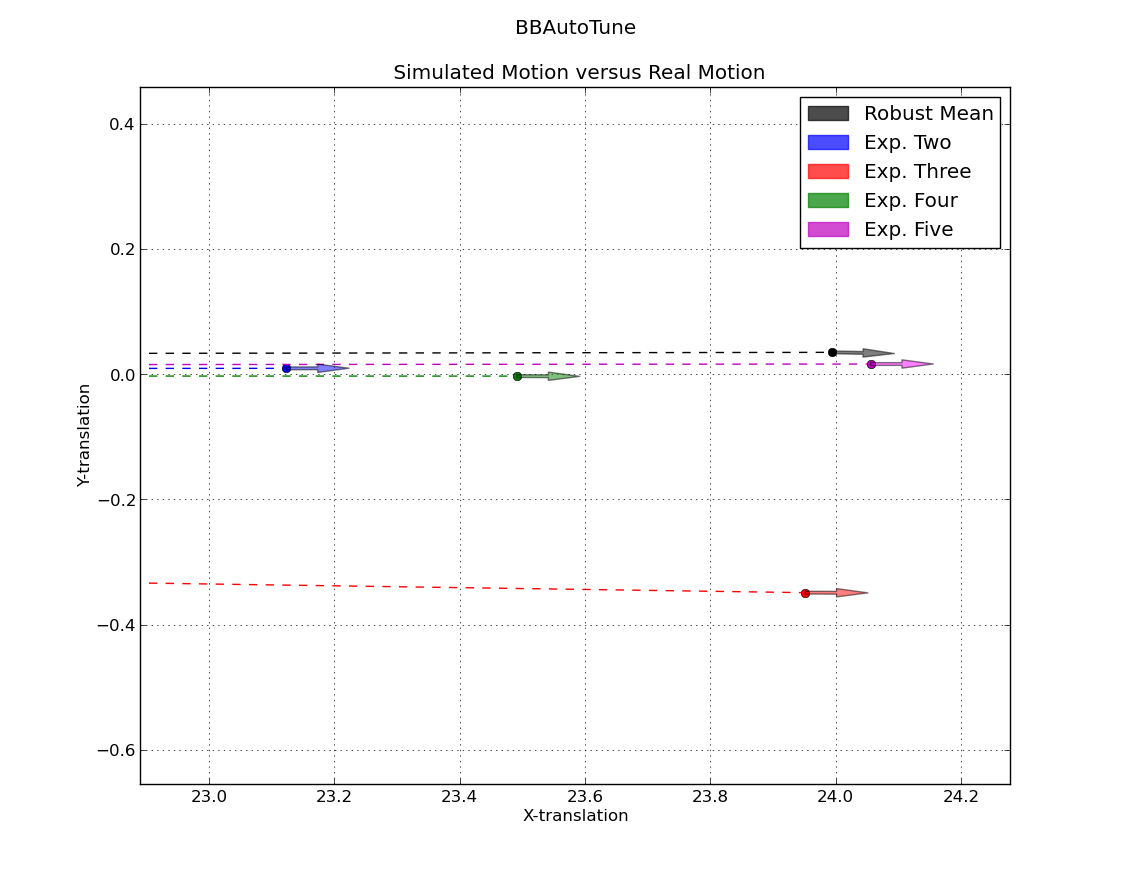
\includegraphics[width=6in]{../Figures/Chapter4/simu_vs_real_line.png}
\rule{35em}{0.5pt}
\caption[Simulated versus Real Motion Line Plot]{The final states of the top phenotypes from experiments two through five compared to the real robot robust mean.}
\label{fig:simu_vs_real_line}
\end{figure}

\begin{figure}[htbp]
\centering
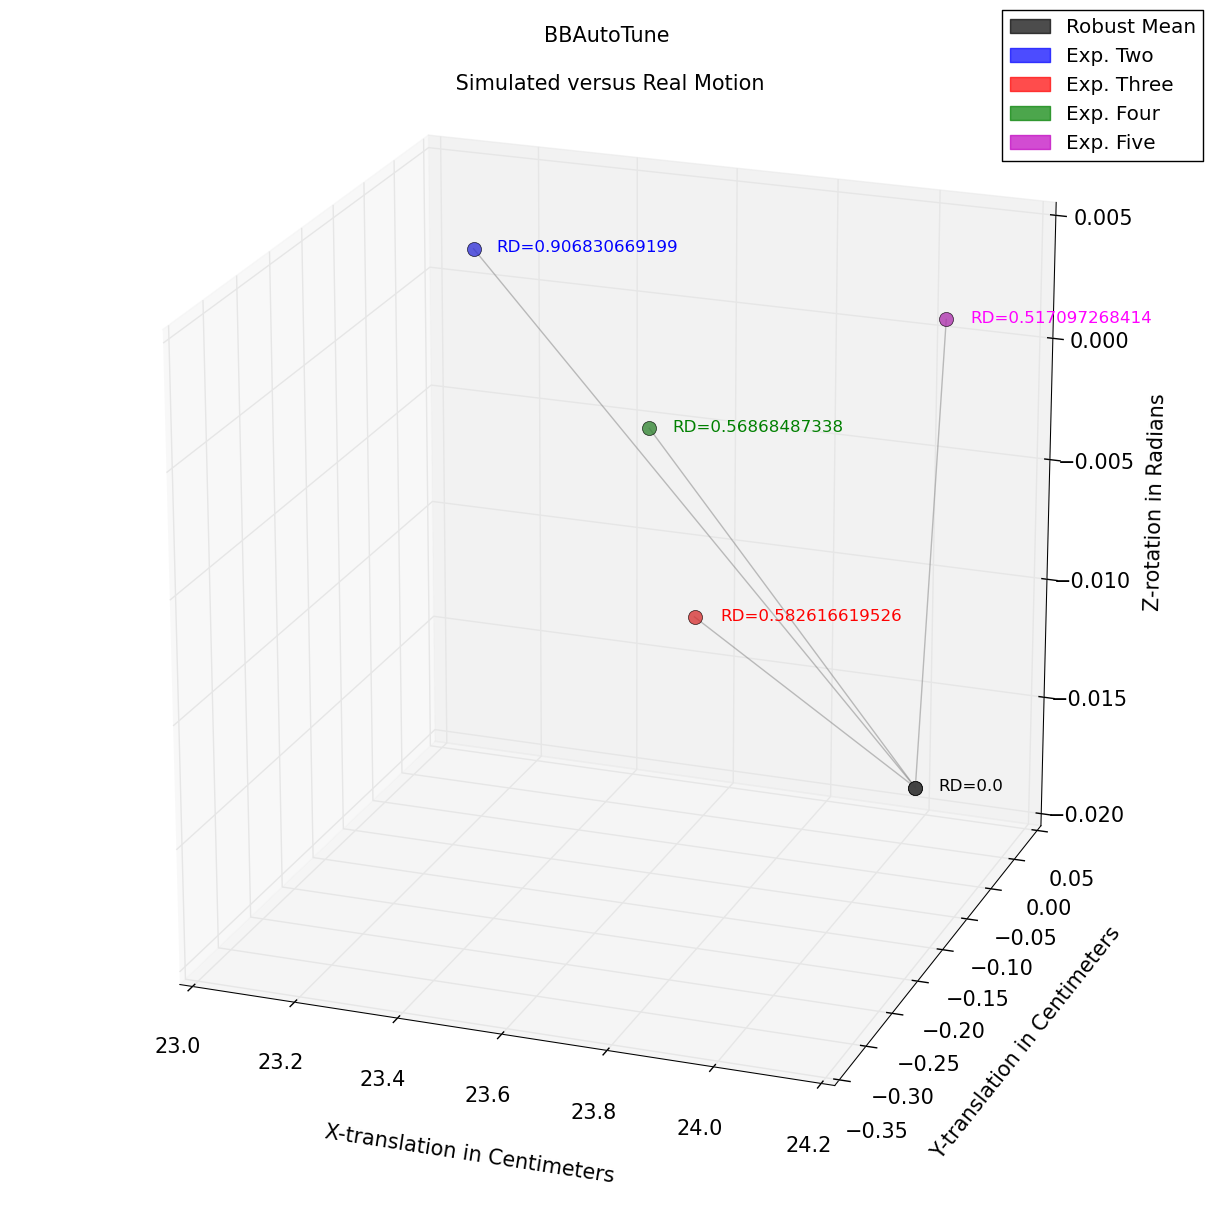
\includegraphics[width=5in]{../Figures/Chapter4/simu_vs_real_3d.png}
\rule{35em}{0.5pt}
\caption[Simulated versus Real Motion 3D Plot]{An alternate view of the final states of the top phenotypes from experiments two through five compared to the real robot robust mean. The robust distances are indicated near each data point.}
\label{fig:simu_vs_real_3d}
\end{figure}

